How do we navigate having two papers from one model without plagiarising ourselves to include the mdoel information also here? Do we just keep it light and reference previous SHAP paper for the model and performance (also have an appendix for the performance of the model for this paper?).

Here we will look at what the SHAP interactions tell us about how the model is making predictions.

\section{Figure 1}

Each patient has a SHAP value per feature to explain how each feature contributes to the model prediction. 
Example of an individual prediction from the model - waterfall plots.

\begin{figure}[!h]
\centering
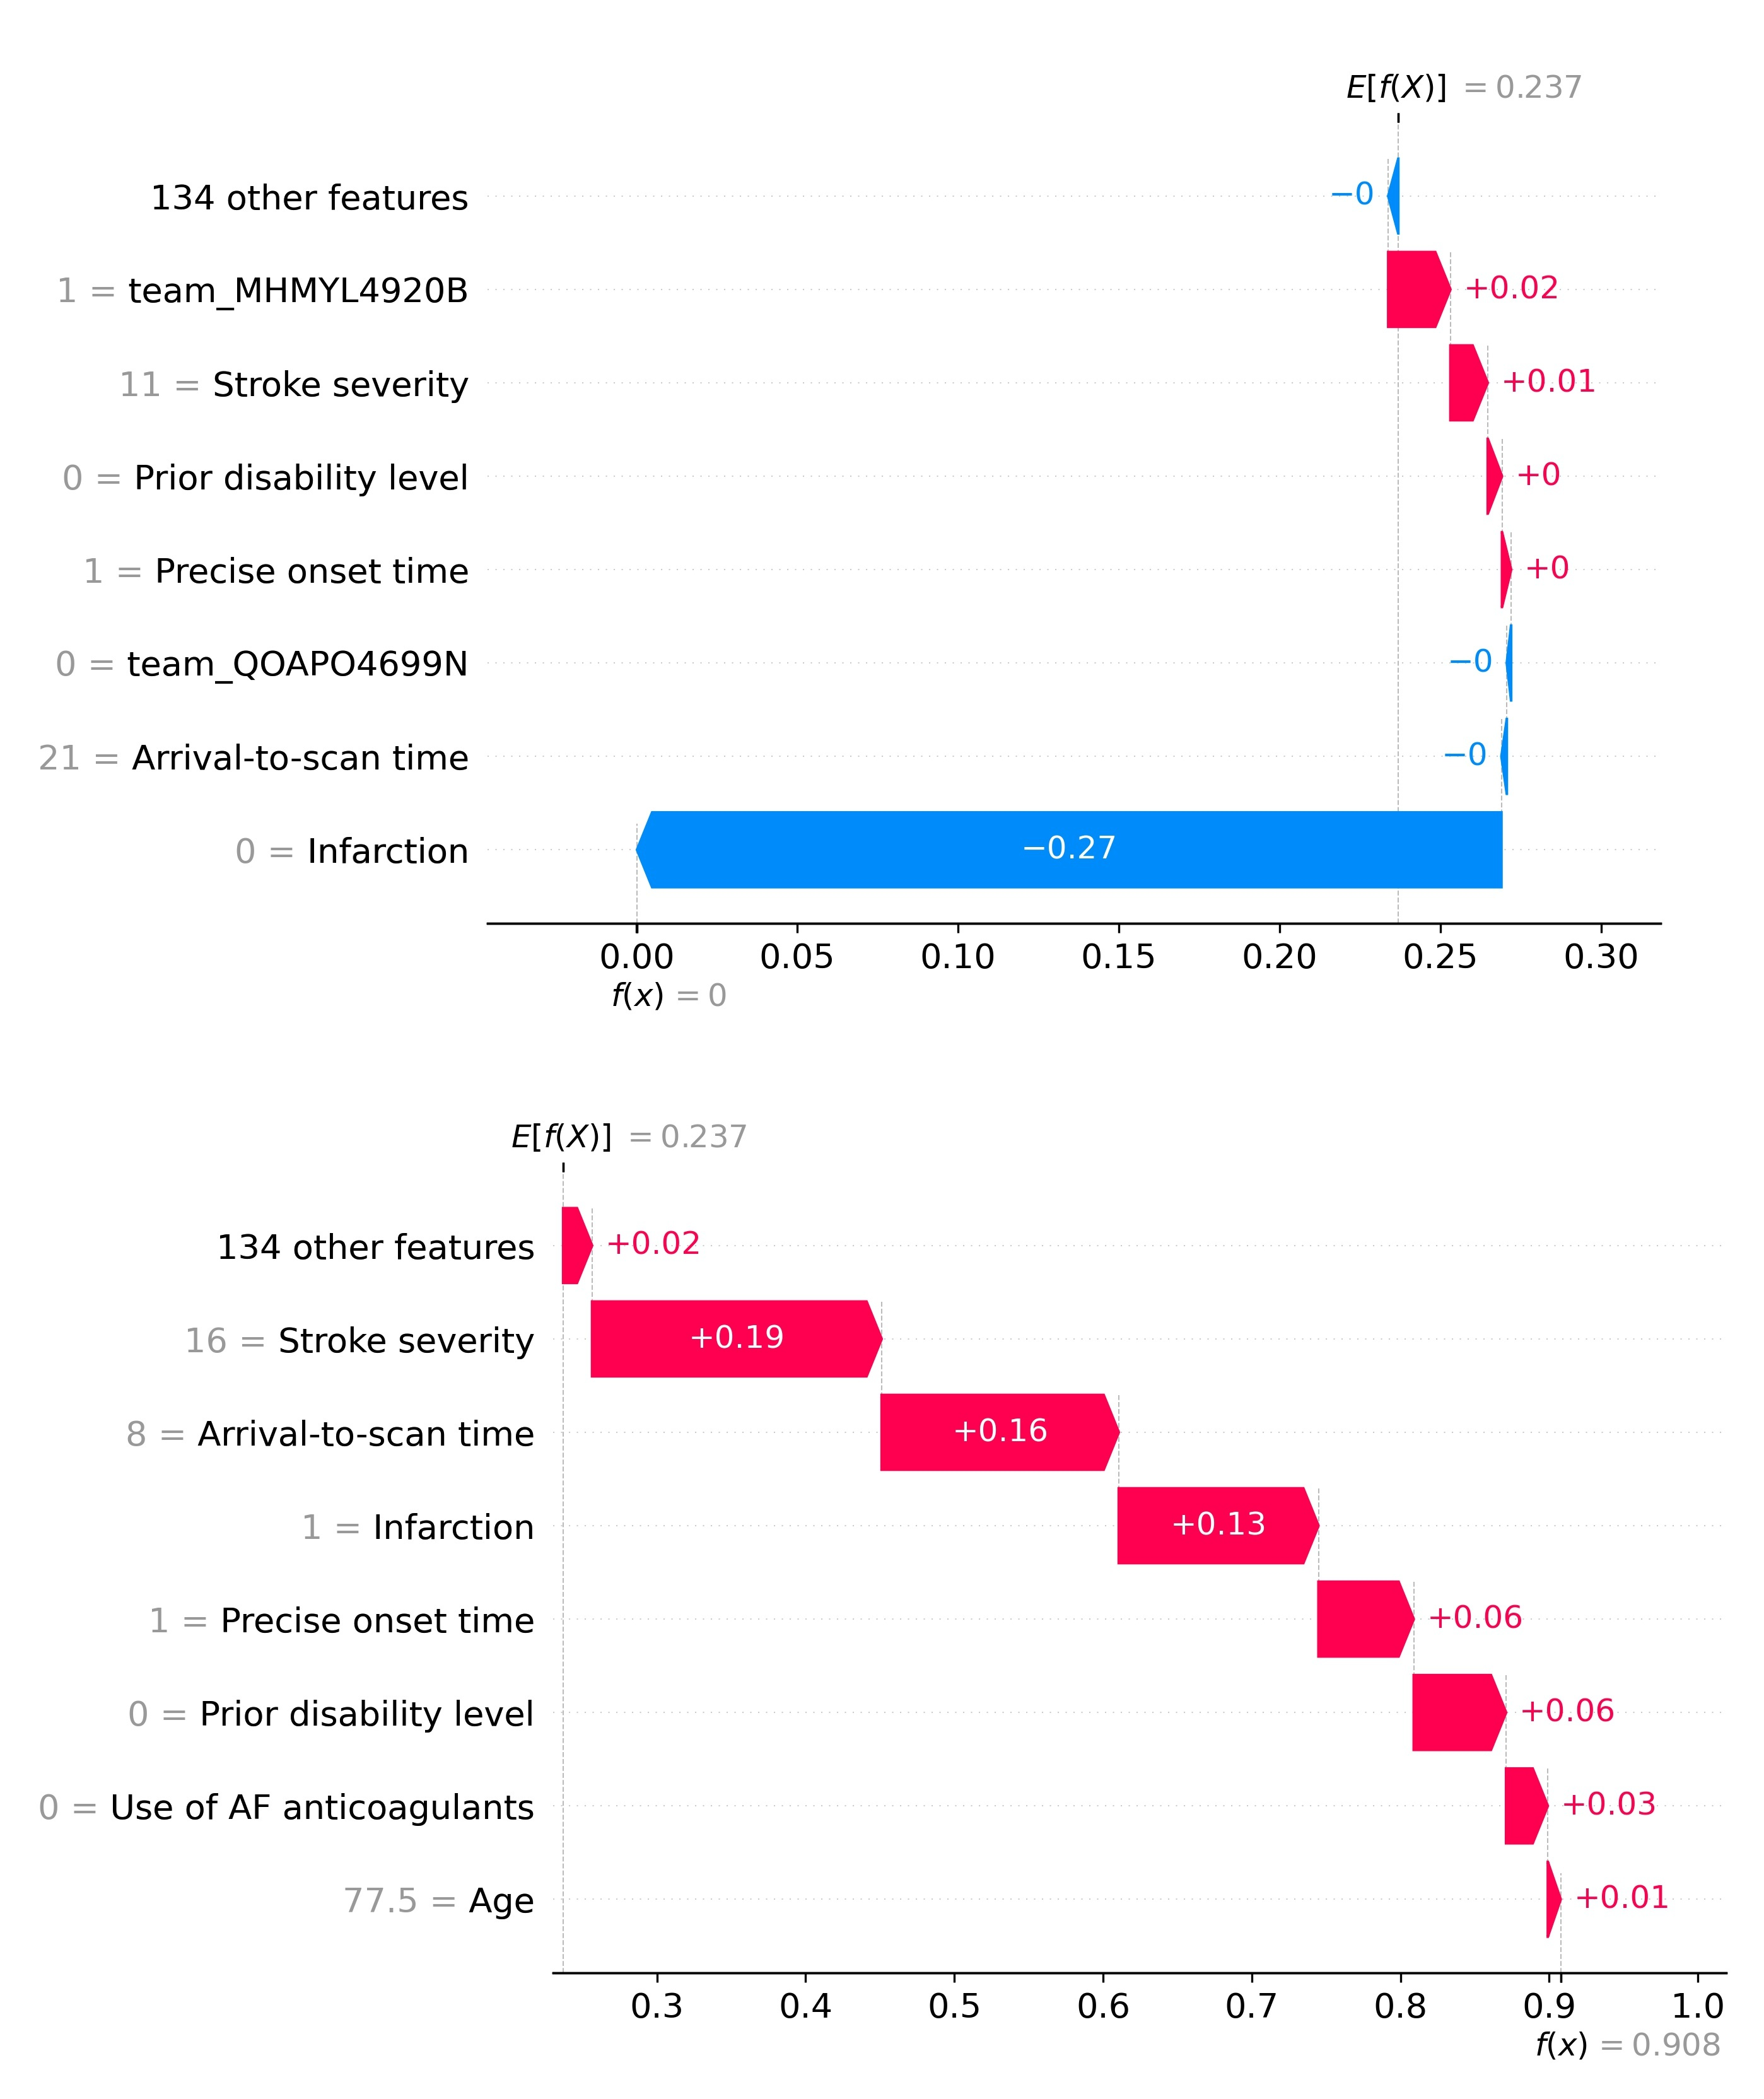
\includegraphics[width=0.75\textwidth]{./images/waterfall}
\caption{}
\label{fig:results_waterfall}
\end{figure}

\newpage
\section{Figure 2}

SHAP plots for the same patient attending 132 different hospitals. The plot shows how each patient feature value contributes to the final prediction of whether that patients is likely to receive thrombolysis.

\begin{figure}[!h]
\centering
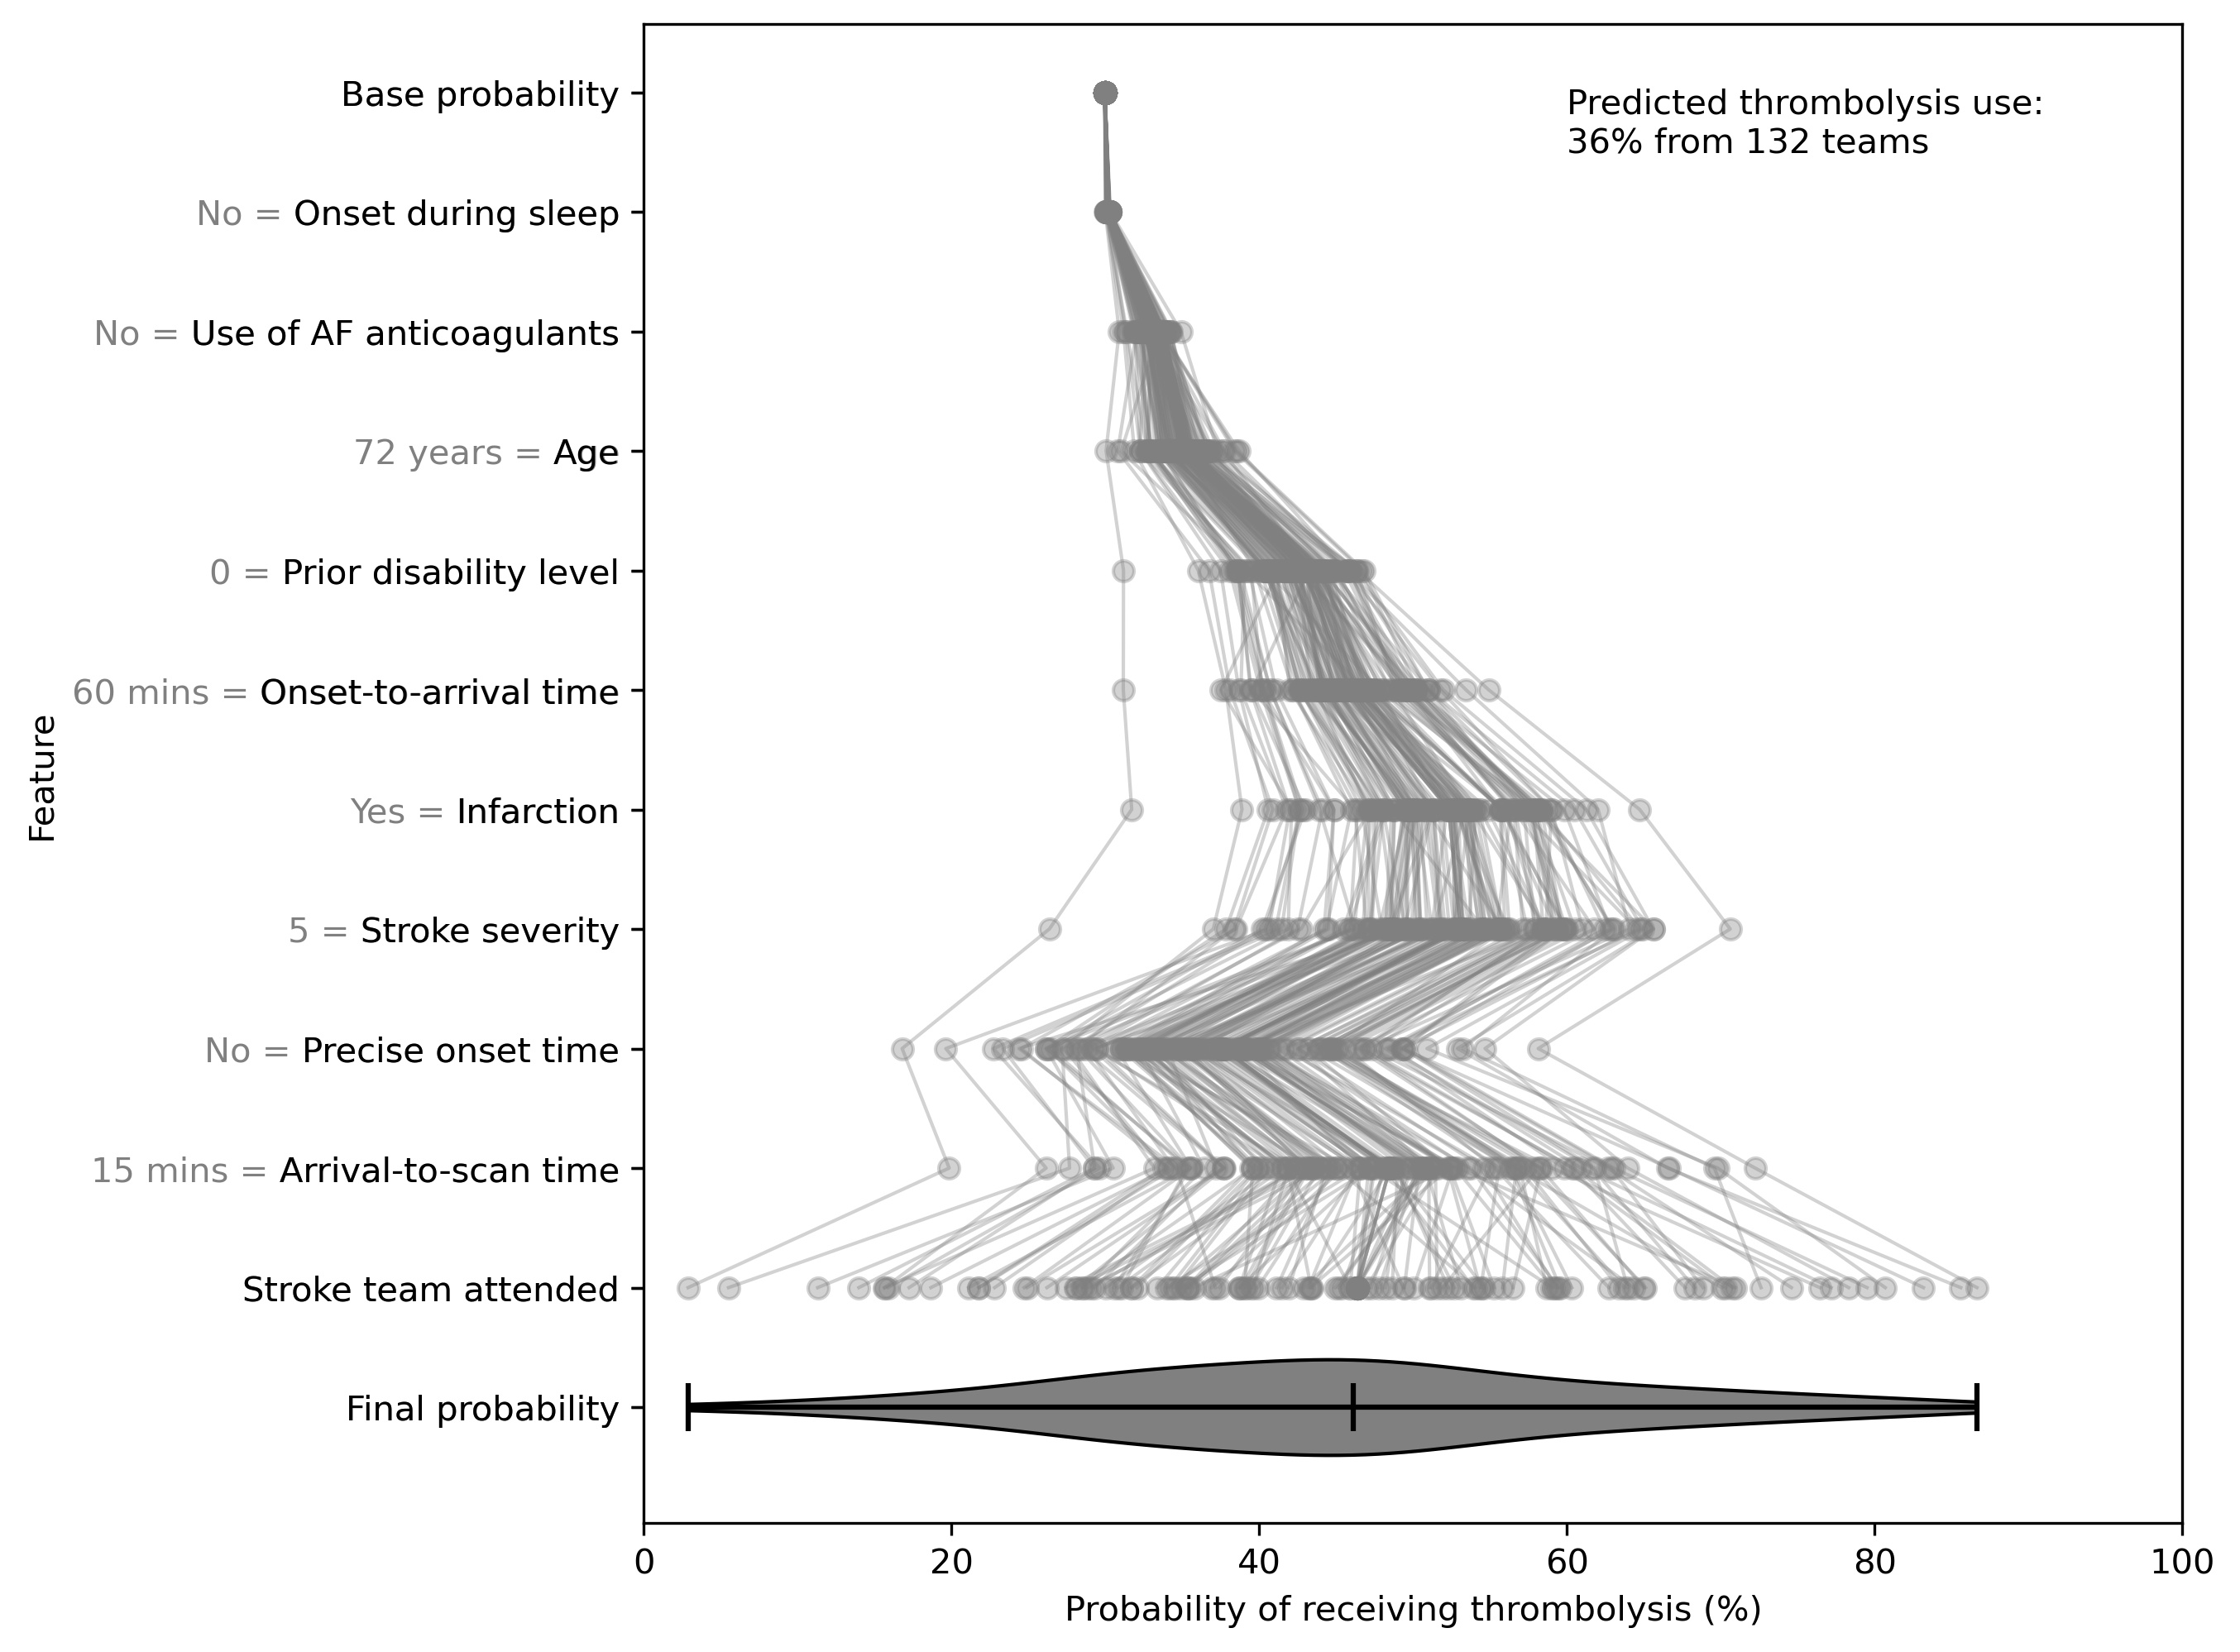
\includegraphics[width=0.75\textwidth]{./images/21_shap_waterfall_with_violin_no_benchmark}
\caption{}
\label{fig:results_11}
\end{figure}

\newpage

\section{Figure 3}

Looking at the population level, the relationship between patient level feature values and their SHAP values.

\begin{figure}[!h]
\centering
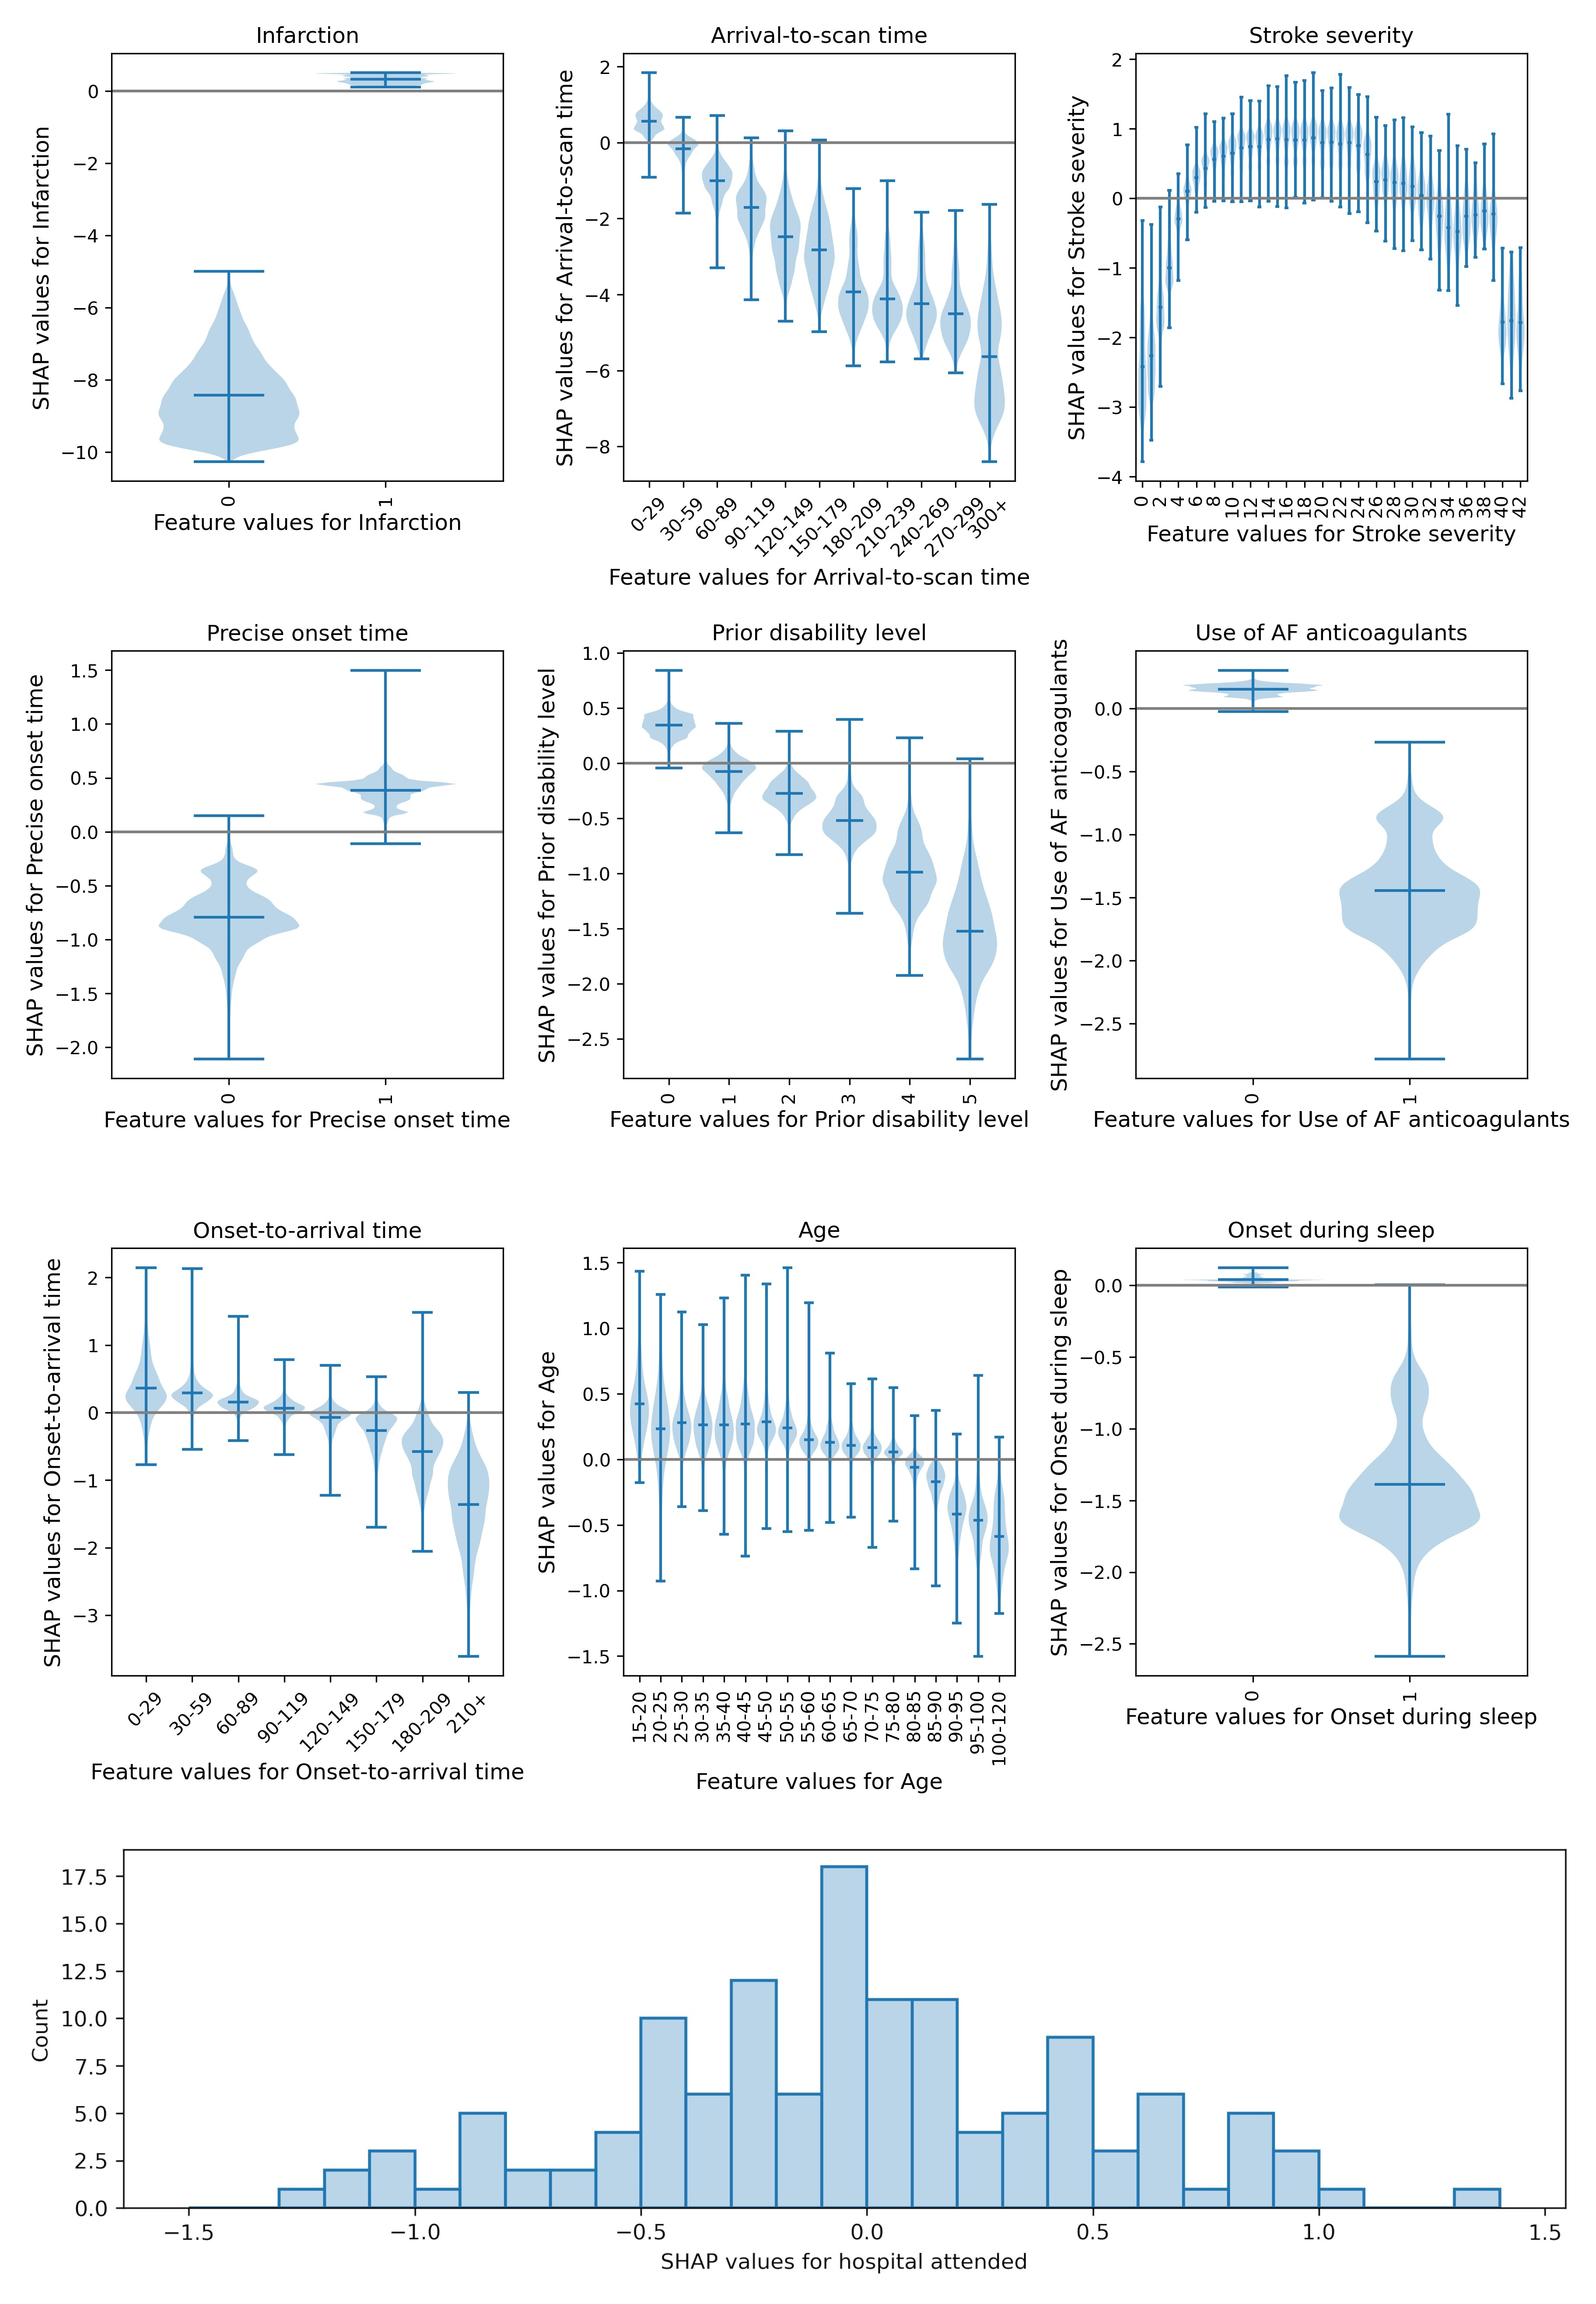
\includegraphics[width=0.75\textwidth]{./images/03a_combined_shap}
\caption{}
\label{fig:results_feature_value_vs}
\end{figure}

\newpage
\section{Figure 4}

The interactions between each feature (on the population level)can be seen using a matrix of dependency plots. Diagonal is the main effect of the feature. The other positions are the interactions between two features.

Shows the interactions between all but the stroke team feature.
\begin{figure}[!h]
\centering
\includegraphics[width=1.0\textwidth]{./images/12a_shap_interactions_scatter}
\caption{}
\label{fig:results_9}
\end{figure}

\newpage

\section{Figure 5}

Each SHAP value is made up of main effect and SHAP interactions.

Adjustment of SHAP main effects by individual hospital. Each row first (left) shows the SHAP main effect of the feature, then (middle) a hospital where the SHAP interaction attenuates the main effect, and finally (right) a hospital where the SHAP interaction strengthens the main effect. Top row (red): SHAP main effect and adjusted SHAP values for precise stroke onset time. Middle row (green): SHAP main effect and adjusted SHAP values for stroke severity. Bottom row (blue): SHAP main effect and adjusted SHAP values for pre-stroke disability

\begin{figure}[!h]
\centering
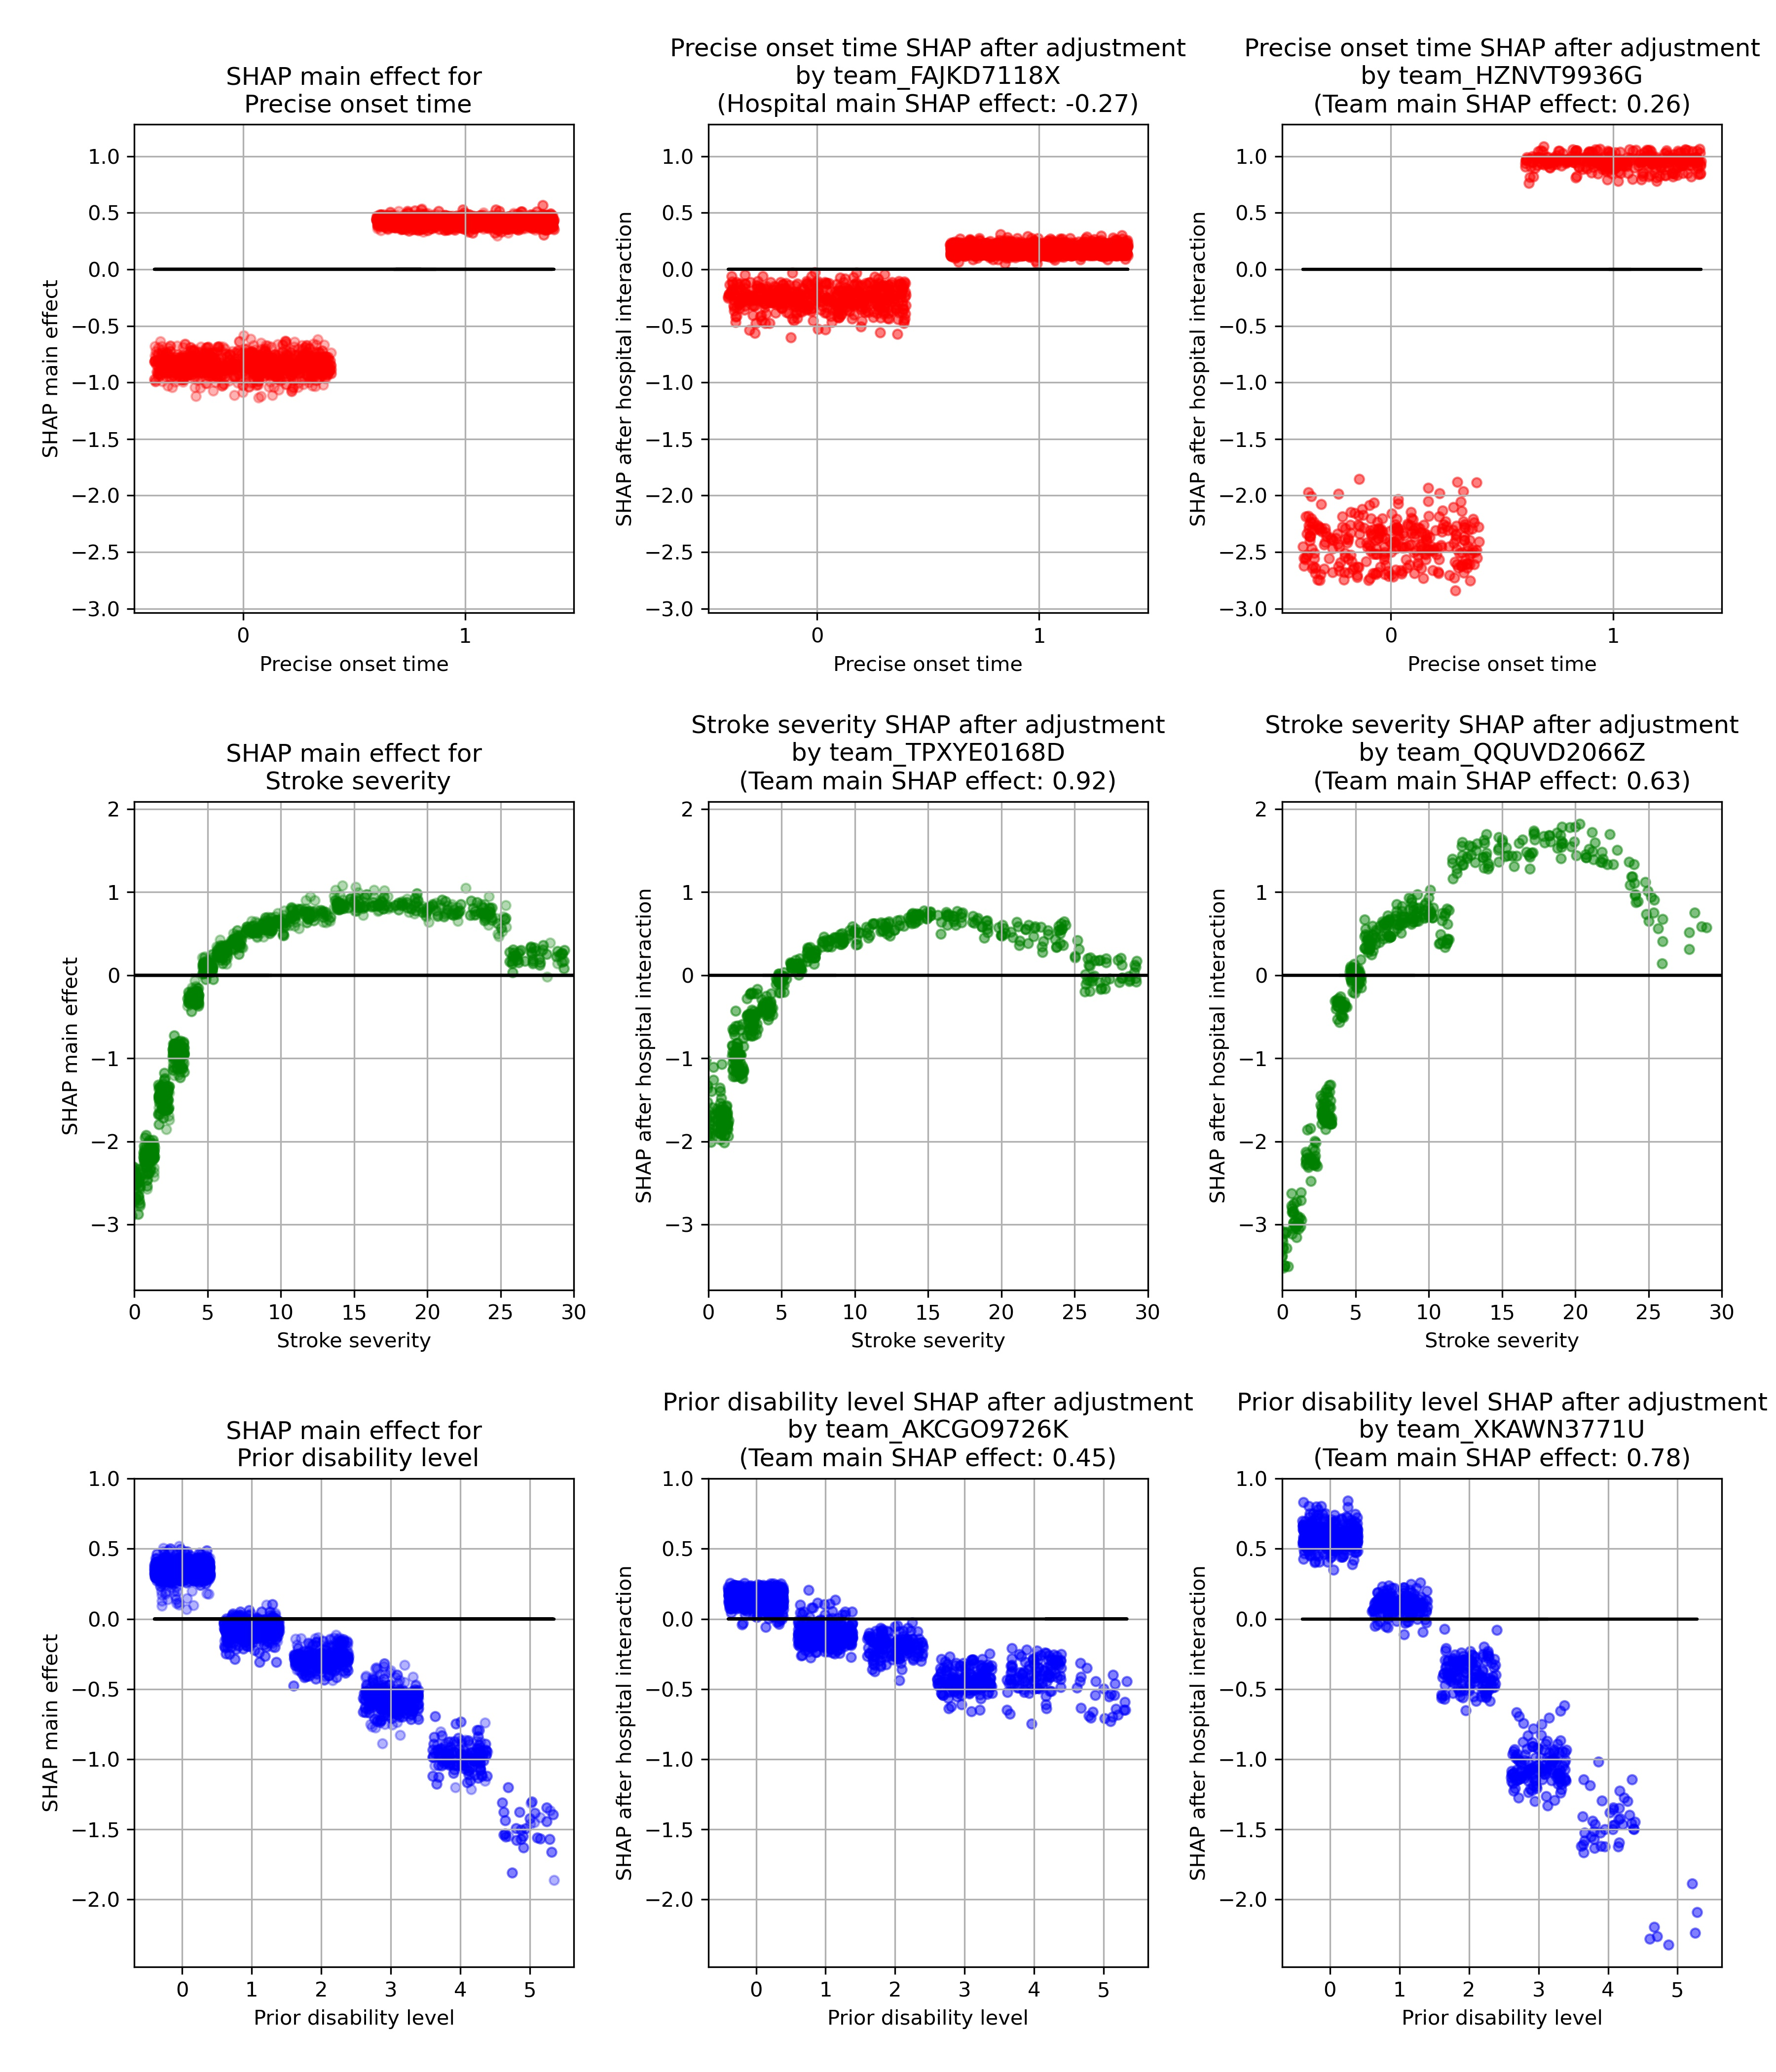
\includegraphics[width=0.8\textwidth]{./images/12aa_three_way_shap_adjustment}
\caption{}
\label{fig:results_2}
\end{figure}

\newpage

\iffalse

    \begin{figure}[!h]
    \centering
    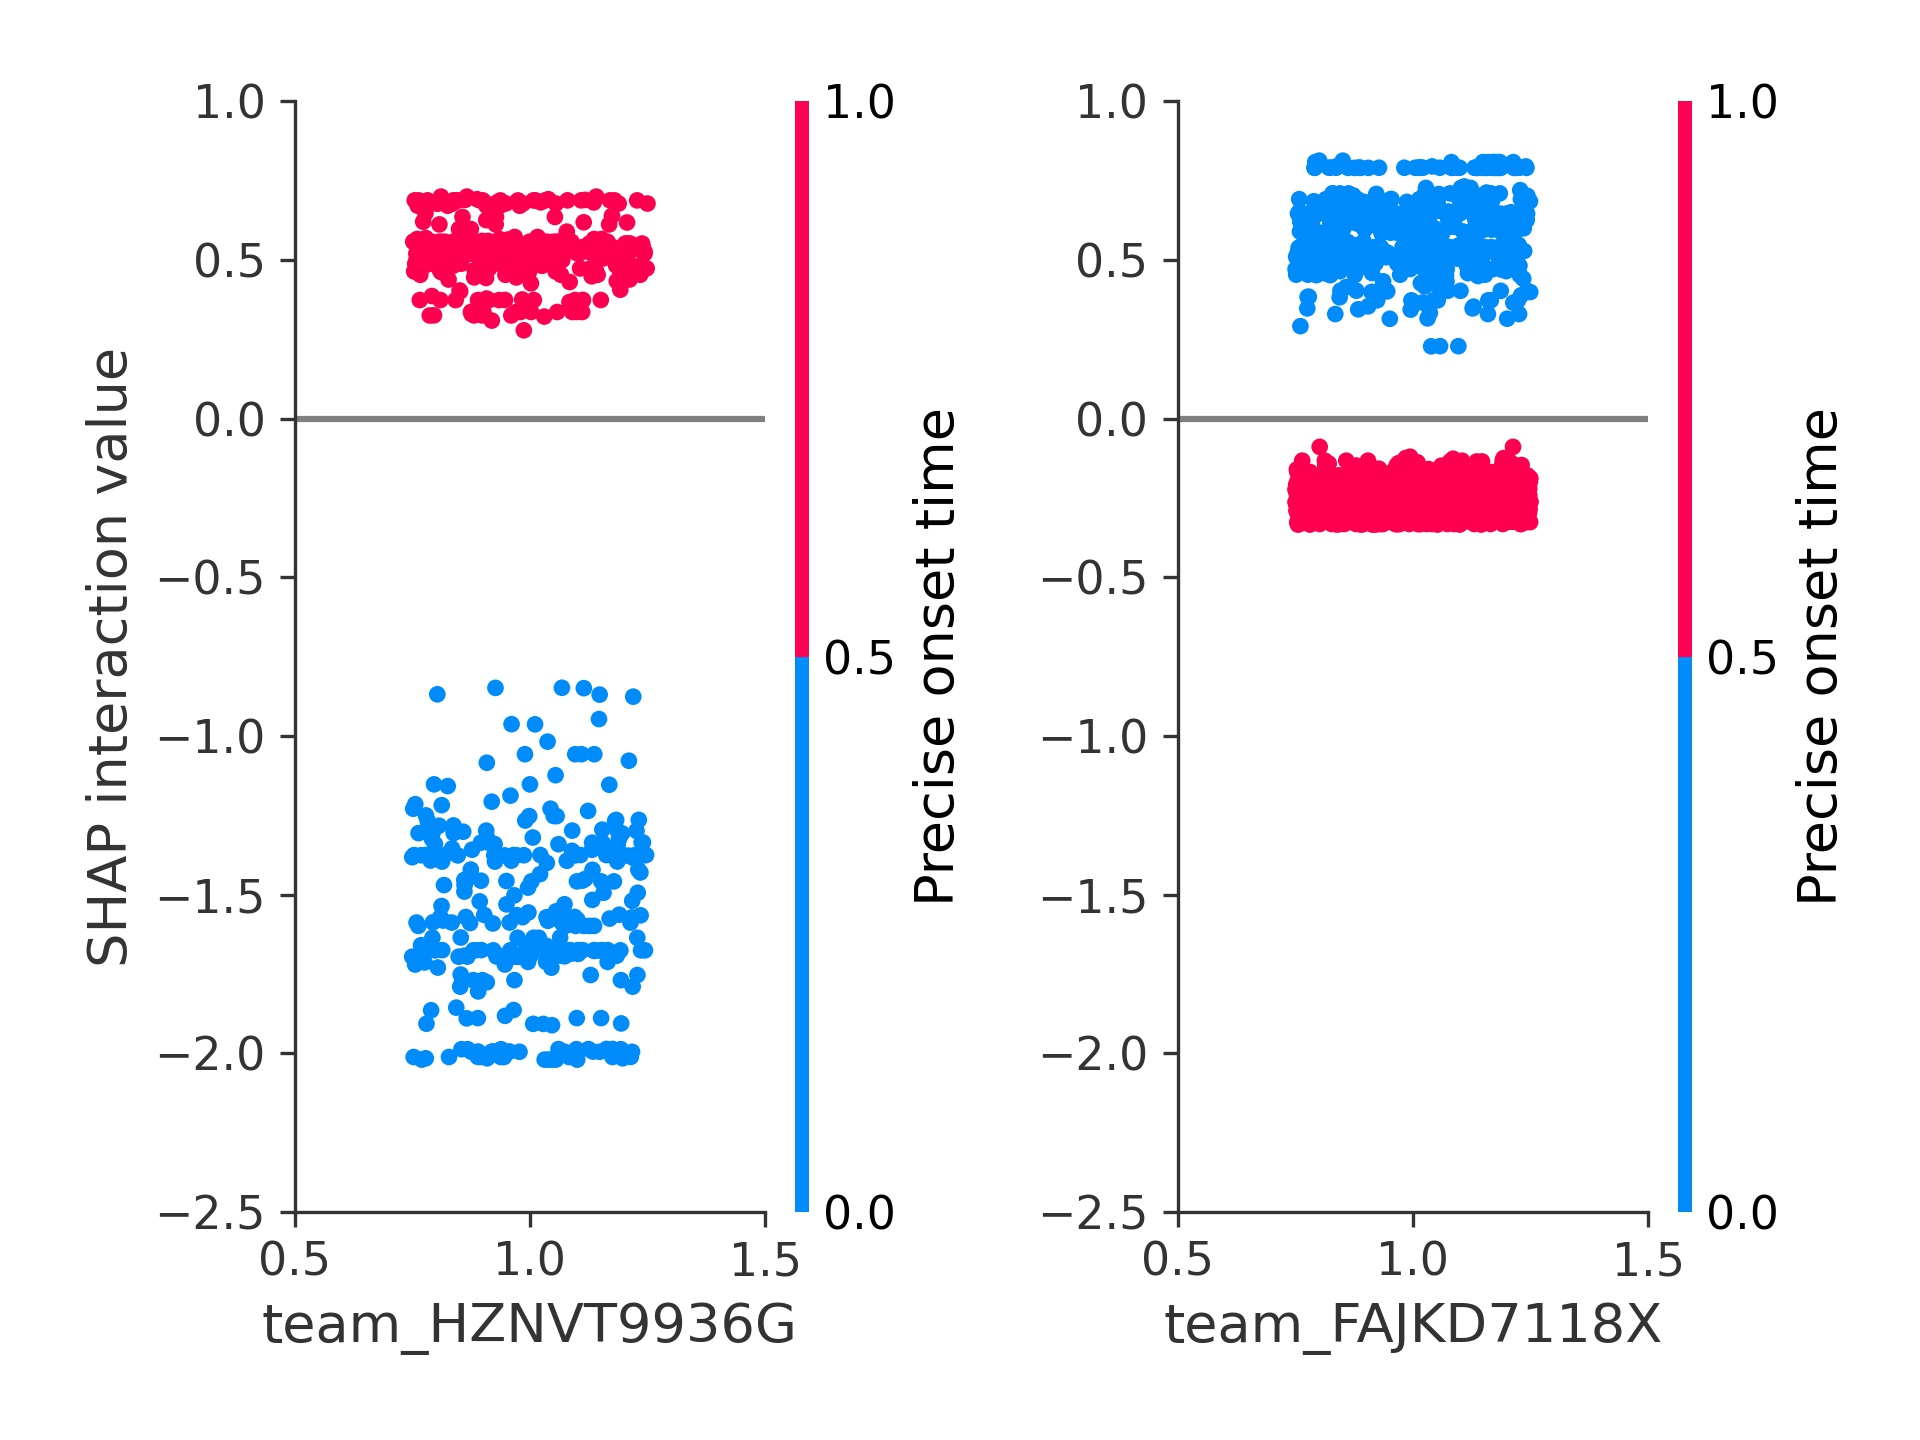
\includegraphics[width=0.75\textwidth]{./images/12aa_onset_time_type_interaction_example}
    \caption{}
    \label{fig:results_1}
    \end{figure}
    
    \newpage
    
    \begin{figure}[!h]
    \centering
    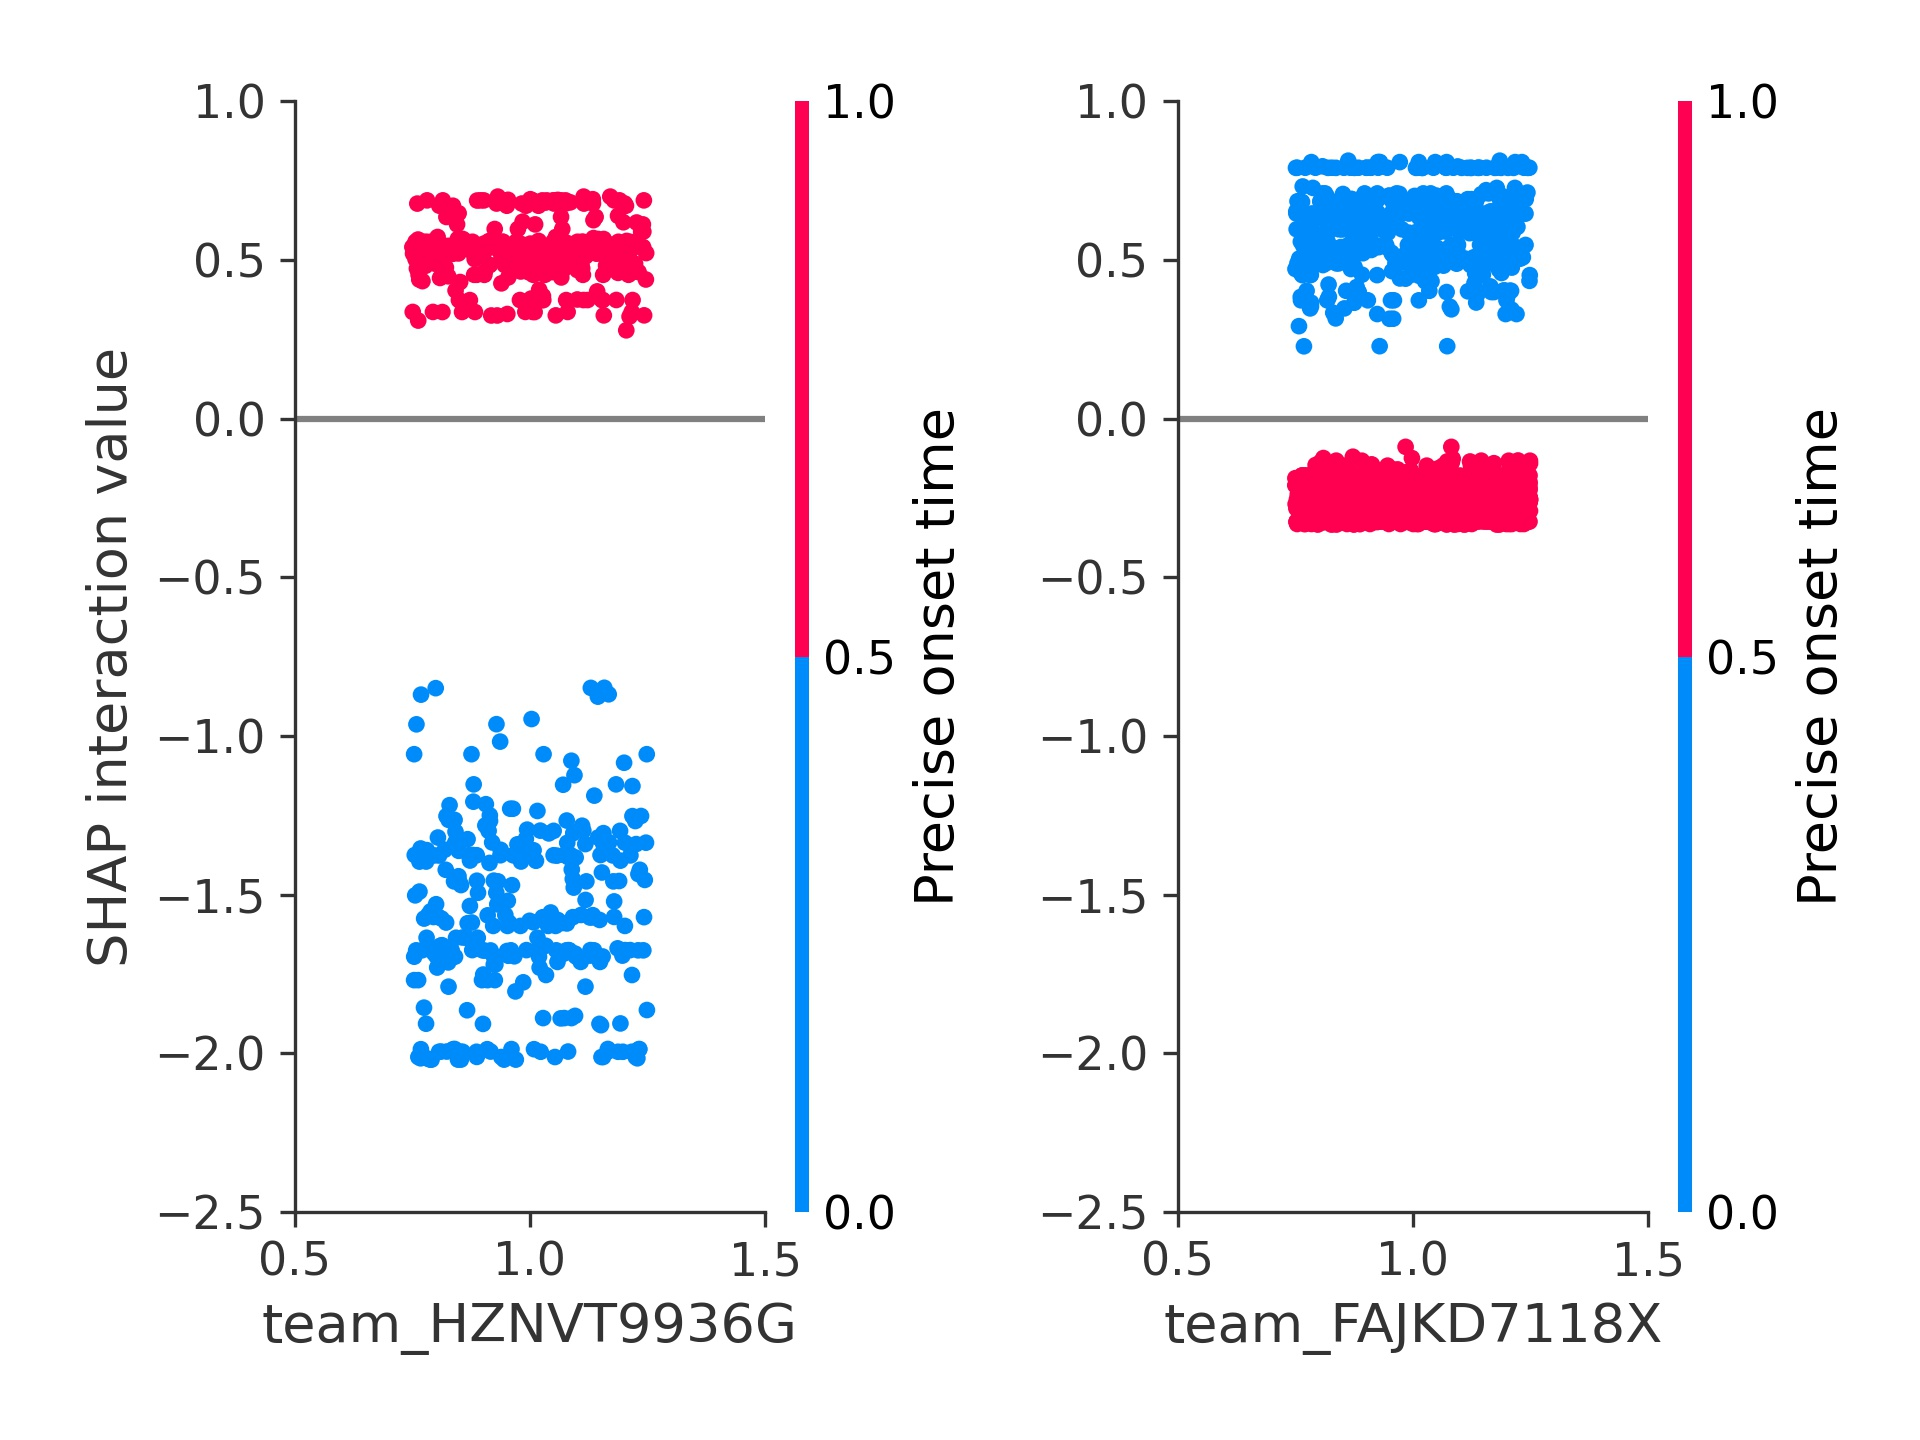
\includegraphics[width=0.75\textwidth]{./images/12aa_xgb_10_features_Precise onset time_interaction_example}
    \caption{}
    \label{fig:results_3}
    \end{figure}
    
    \newpage
    
    \begin{figure}[!h]
    \centering
    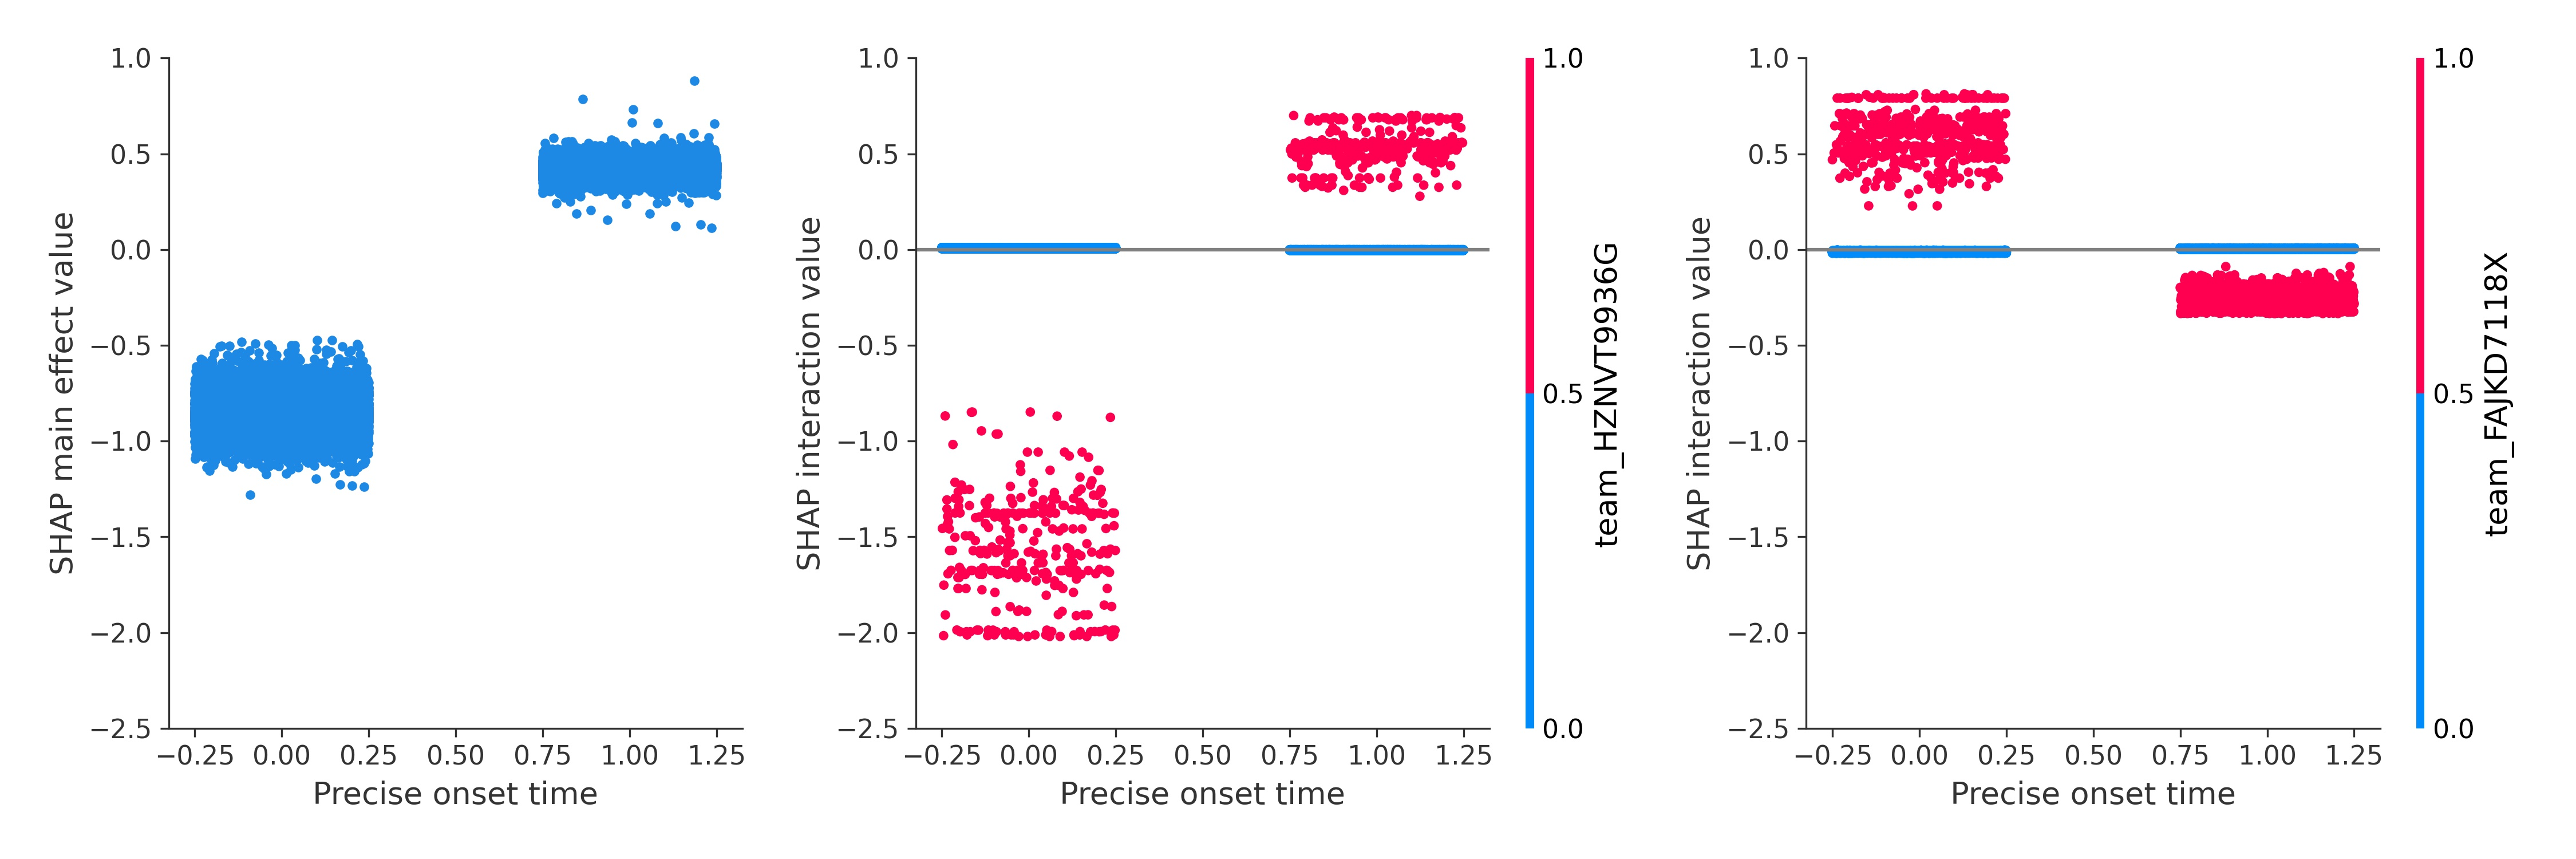
\includegraphics[width=0.75\textwidth]{./images/12aa_xgb_10_features_Precise onset time_interaction_example_with_main_effect}
    \caption{}
    \label{fig:results_4}
    \end{figure}
    
    \newpage
    
    \begin{figure}[!h]
    \centering
    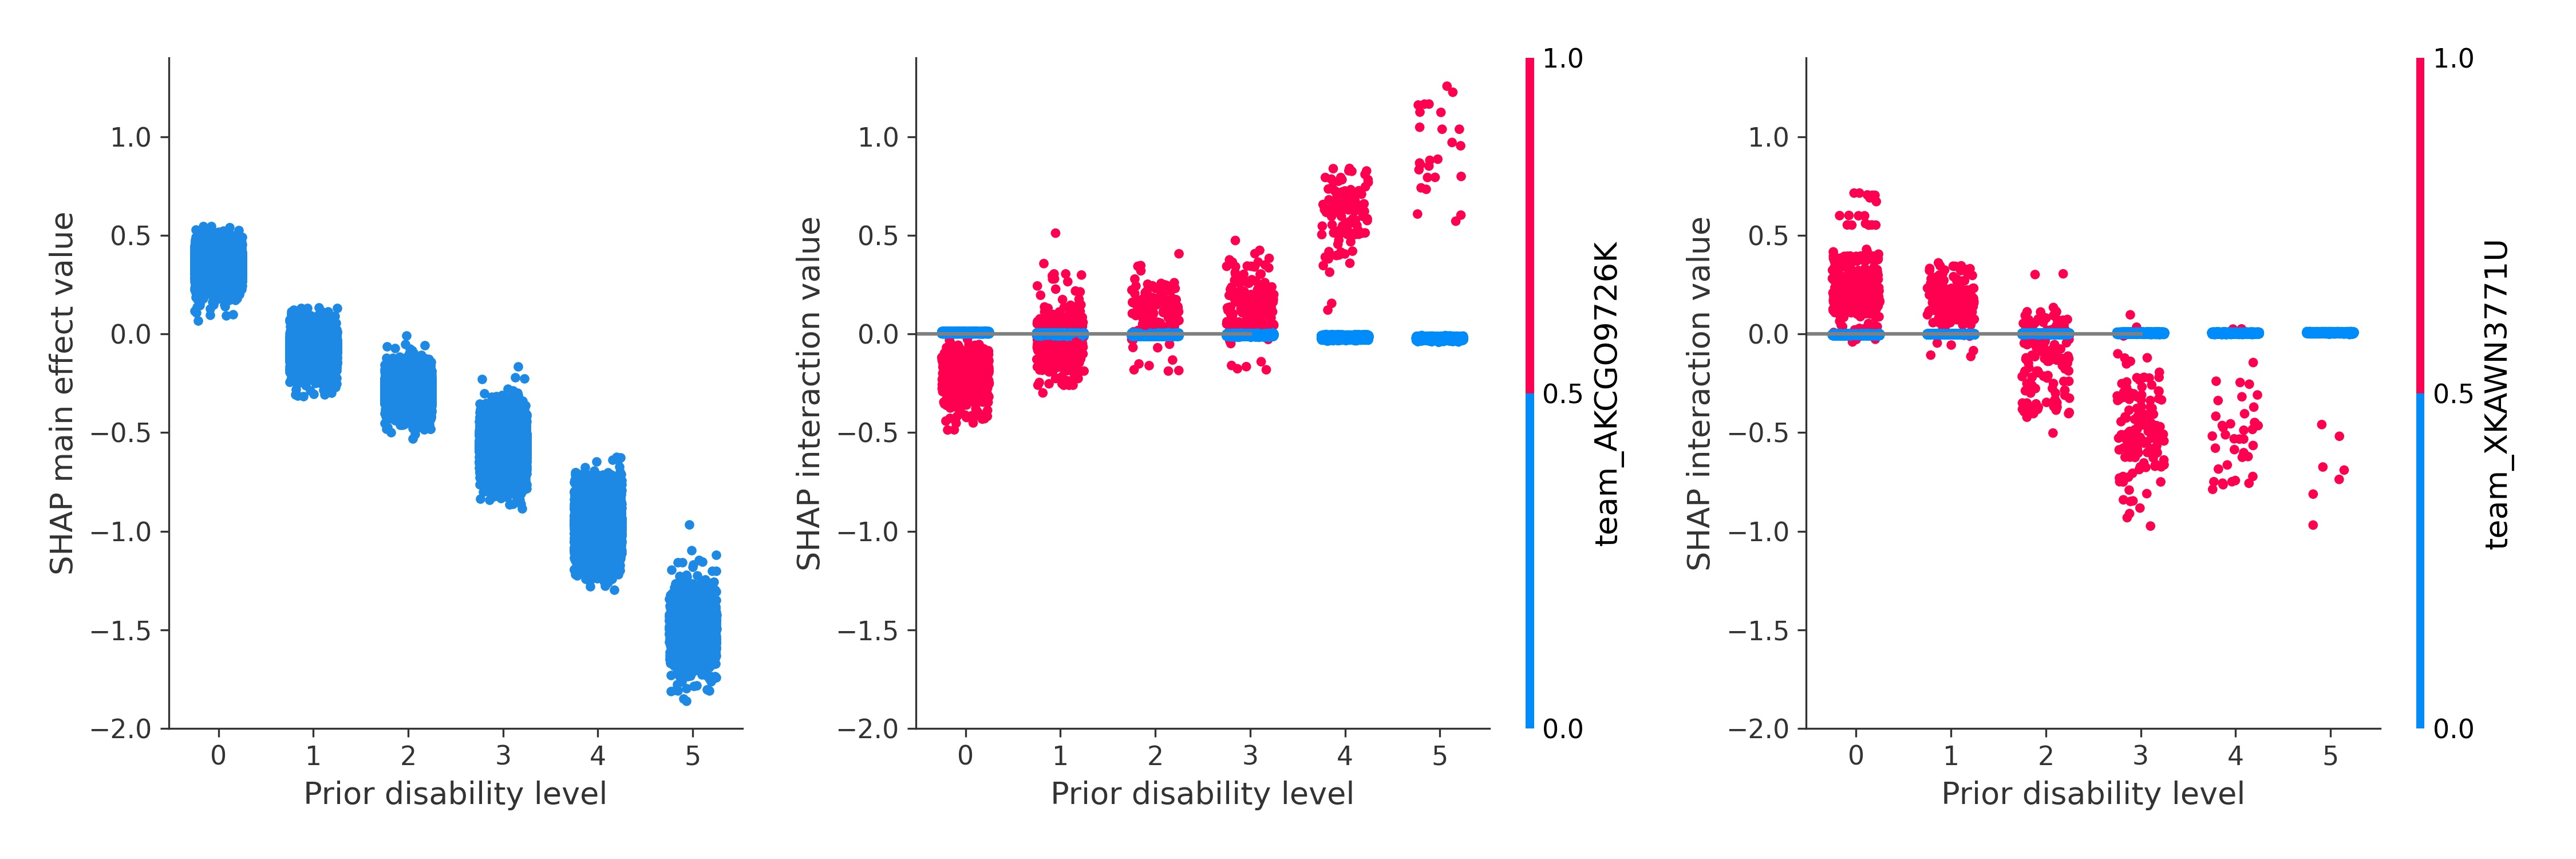
\includegraphics[width=0.75\textwidth]{./images/12aa_xgb_10_features_Prior disability level_interaction_example_with_main_effect}
    \caption{}
    \label{fig:results_5}
    \end{figure}
    
    \newpage
    
    \begin{figure}[!h]
    \centering
    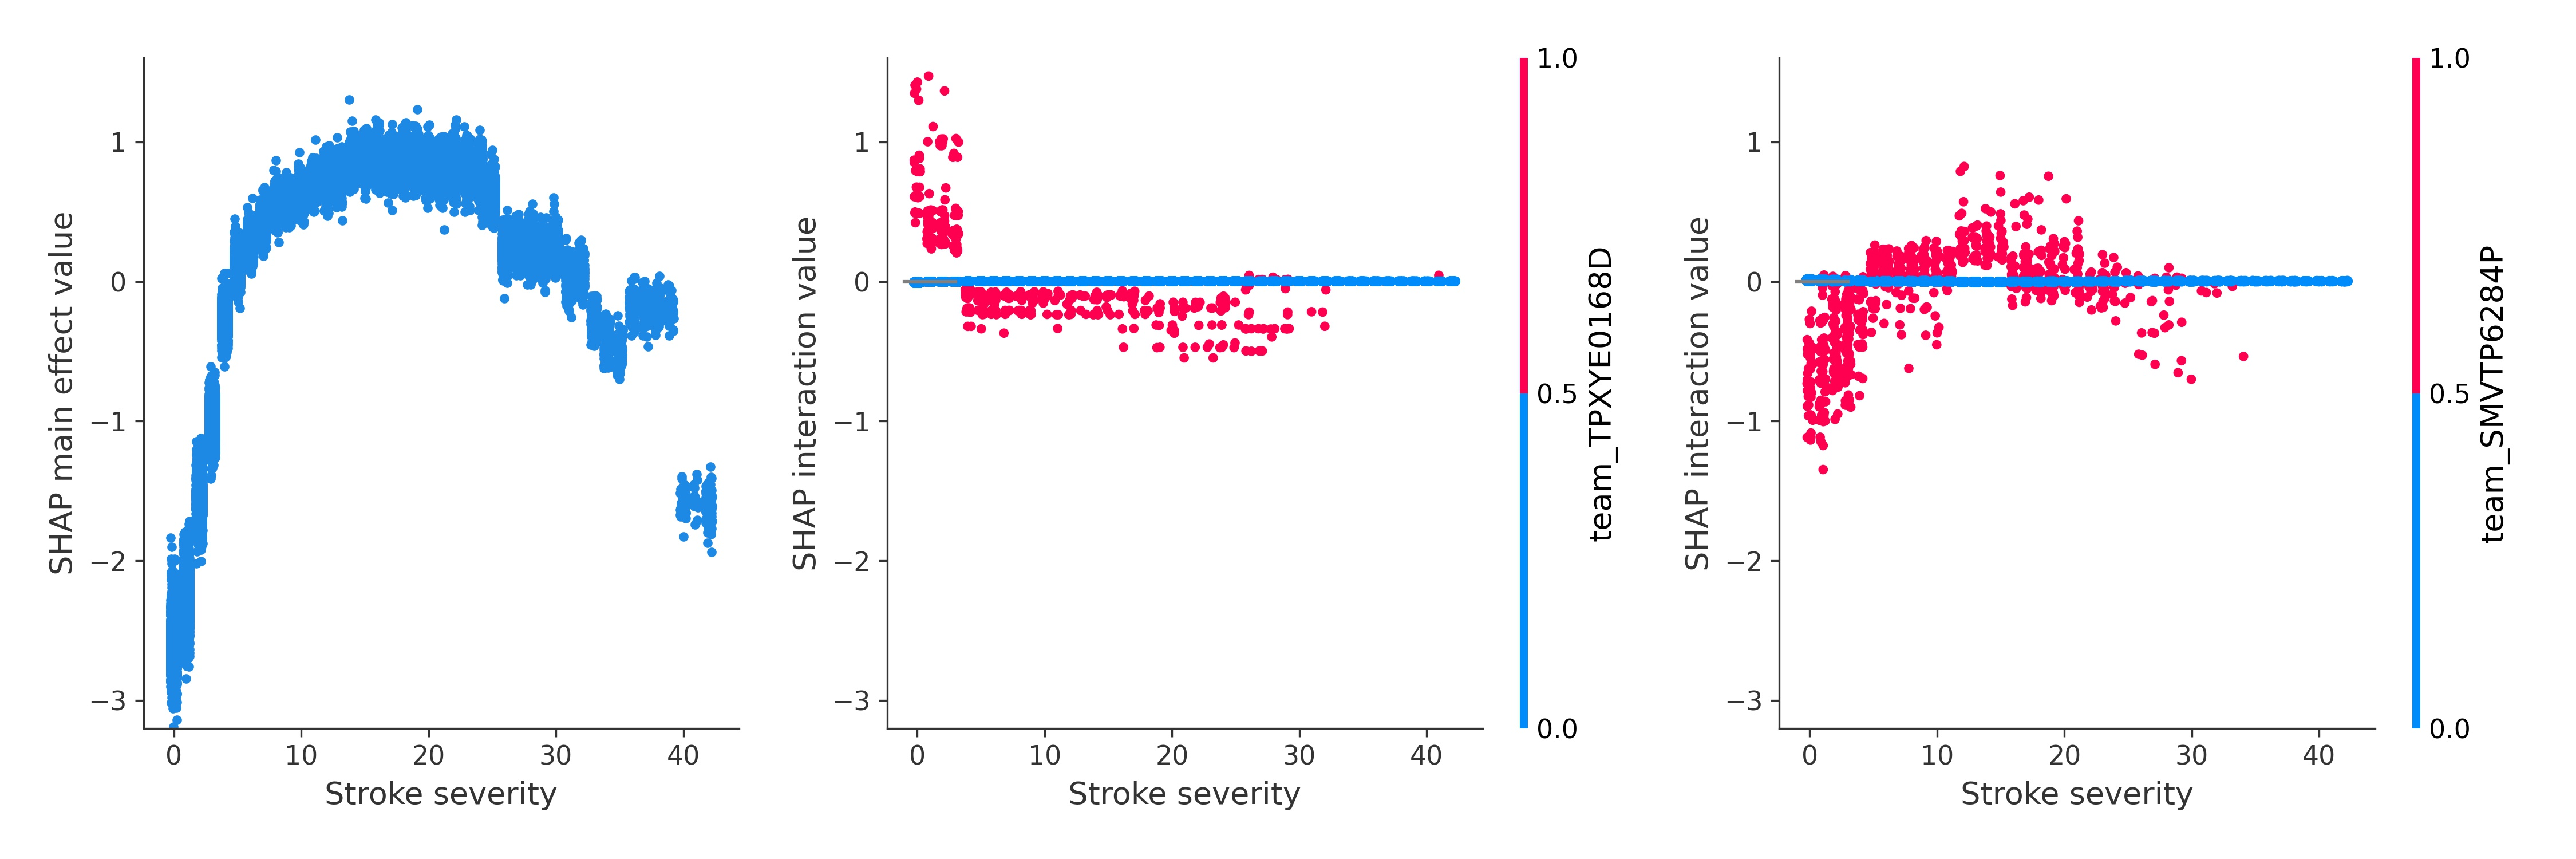
\includegraphics[width=0.75\textwidth]{./images/12aa_xgb_10_features_Stroke severity_interaction_example_with_main_effect}
    \caption{}
    \label{fig:results_6}
    \end{figure}
    
    \newpage
    
    \begin{figure}[!h]
    \centering
    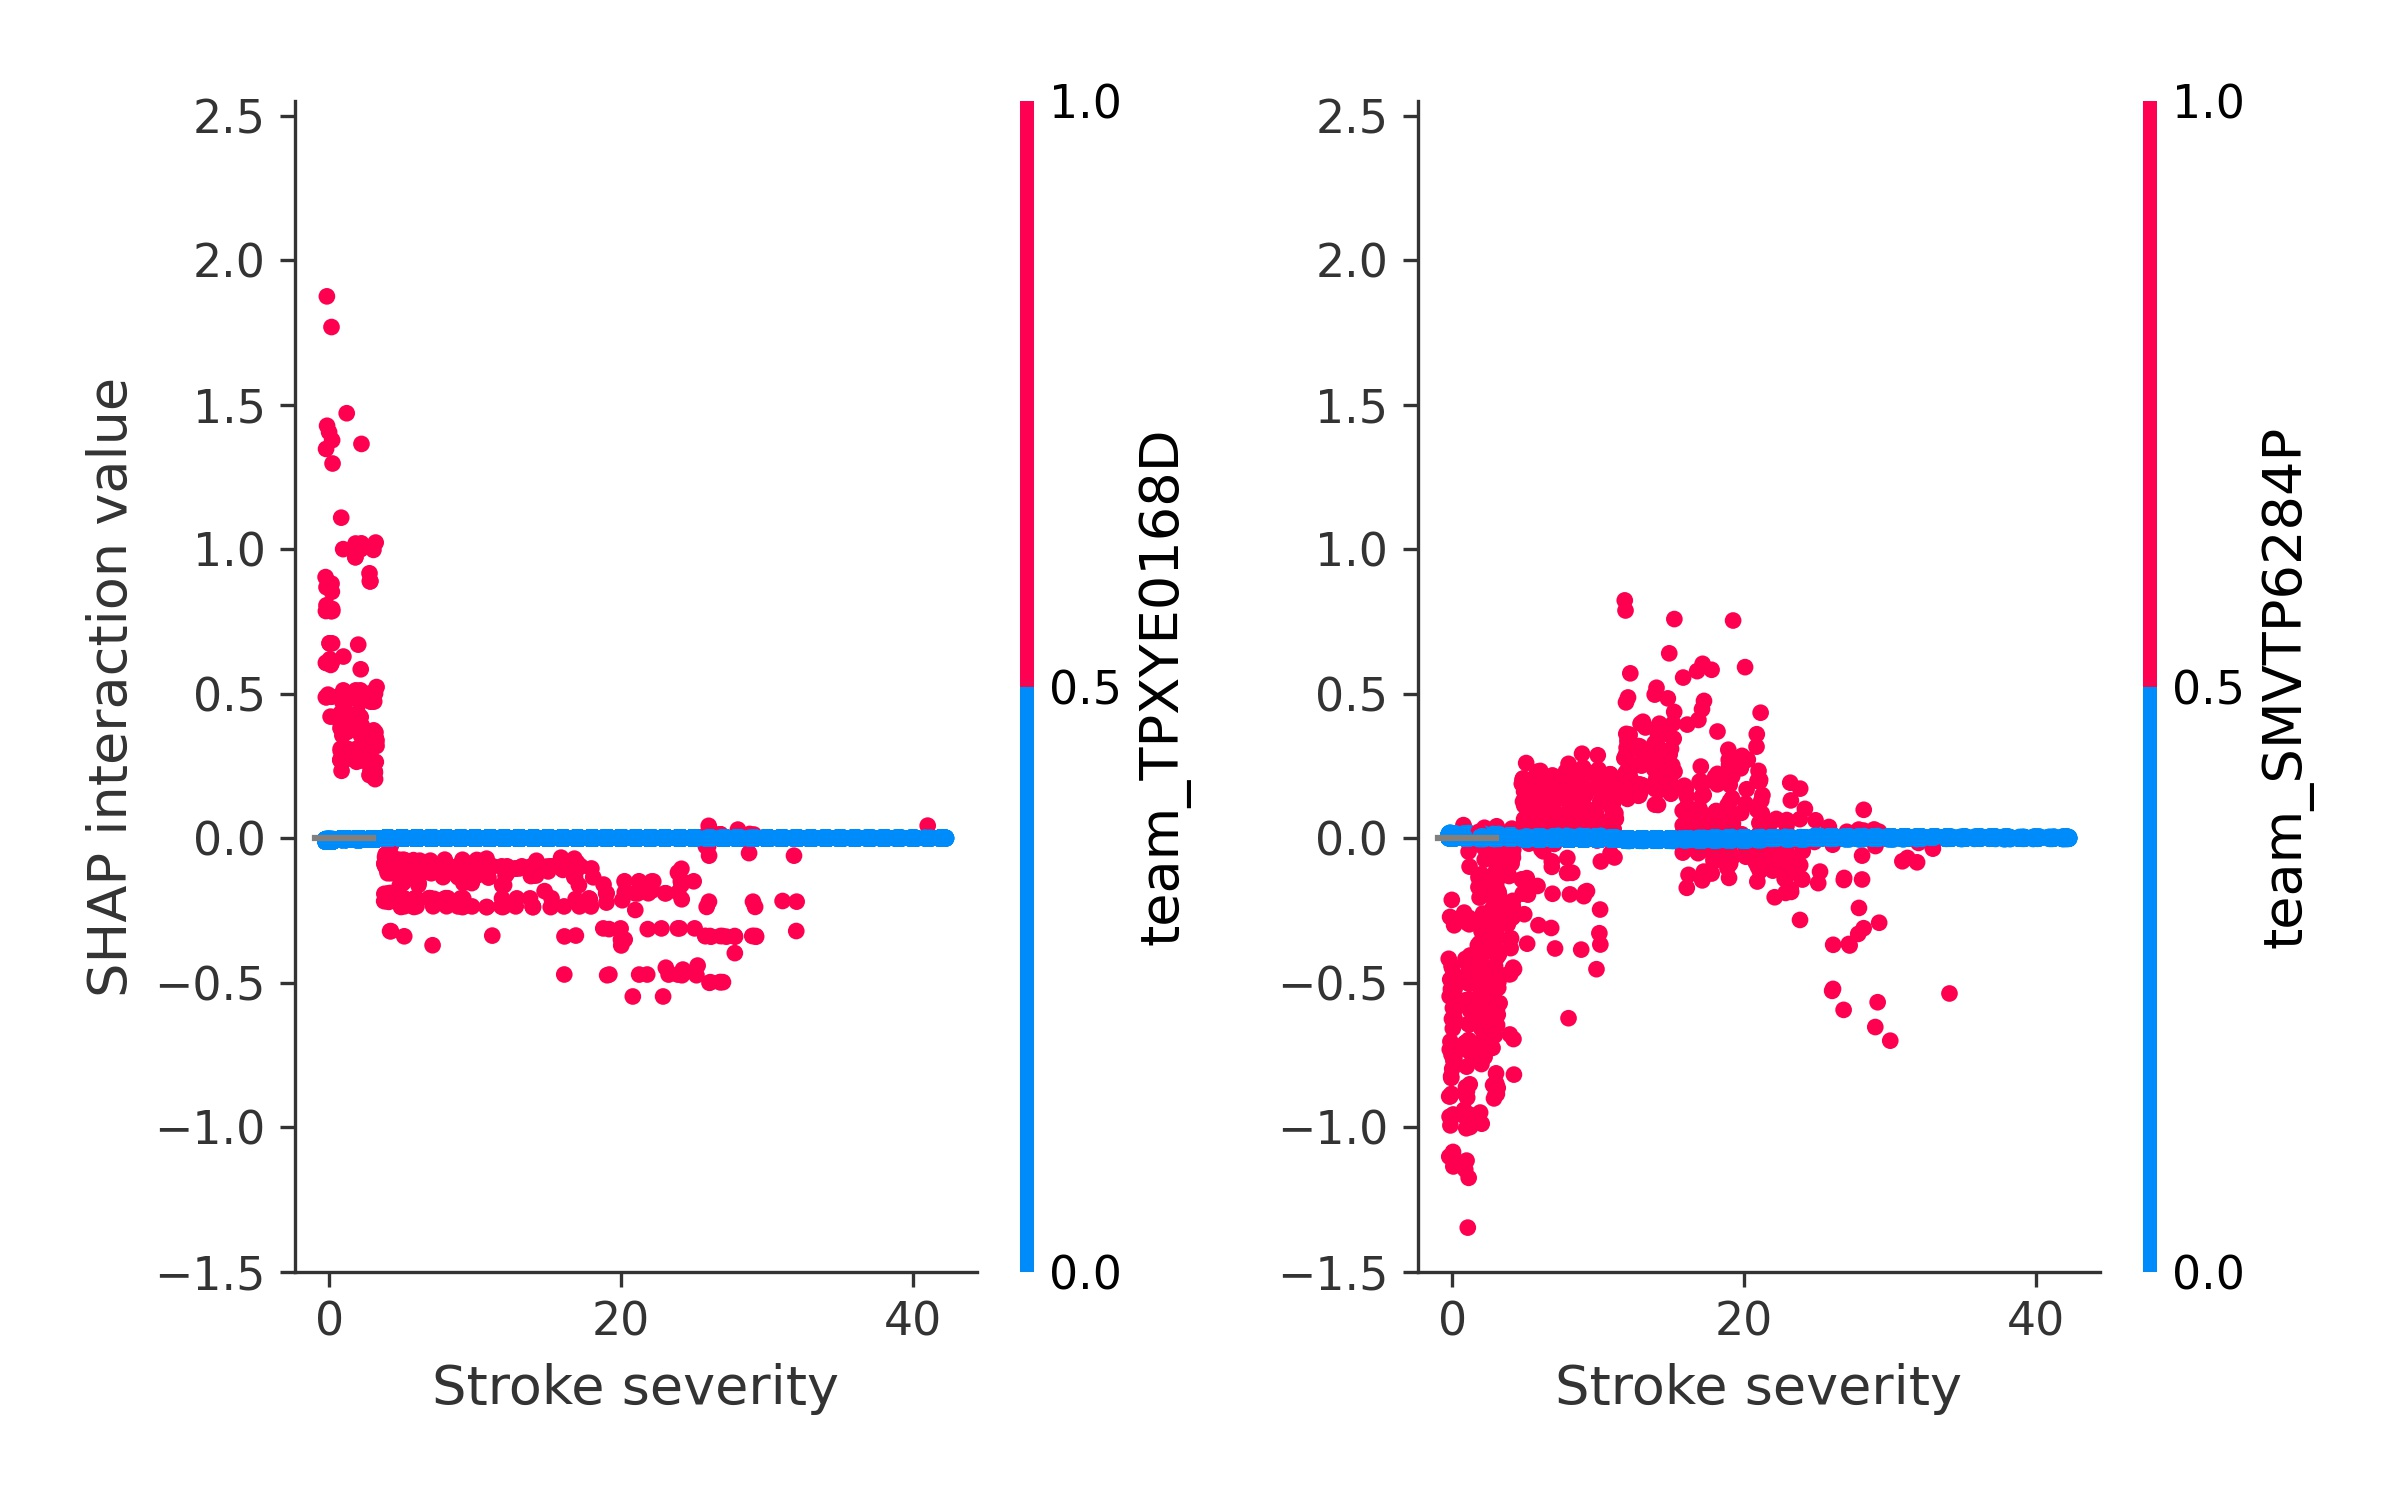
\includegraphics[width=0.75\textwidth]{./images/12ab_stroke_severity_interaction_example}
    \caption{}
    \label{fig:results_7}
    \end{figure}
    
    \newpage
    
    \begin{figure}[!h]
    \centering
    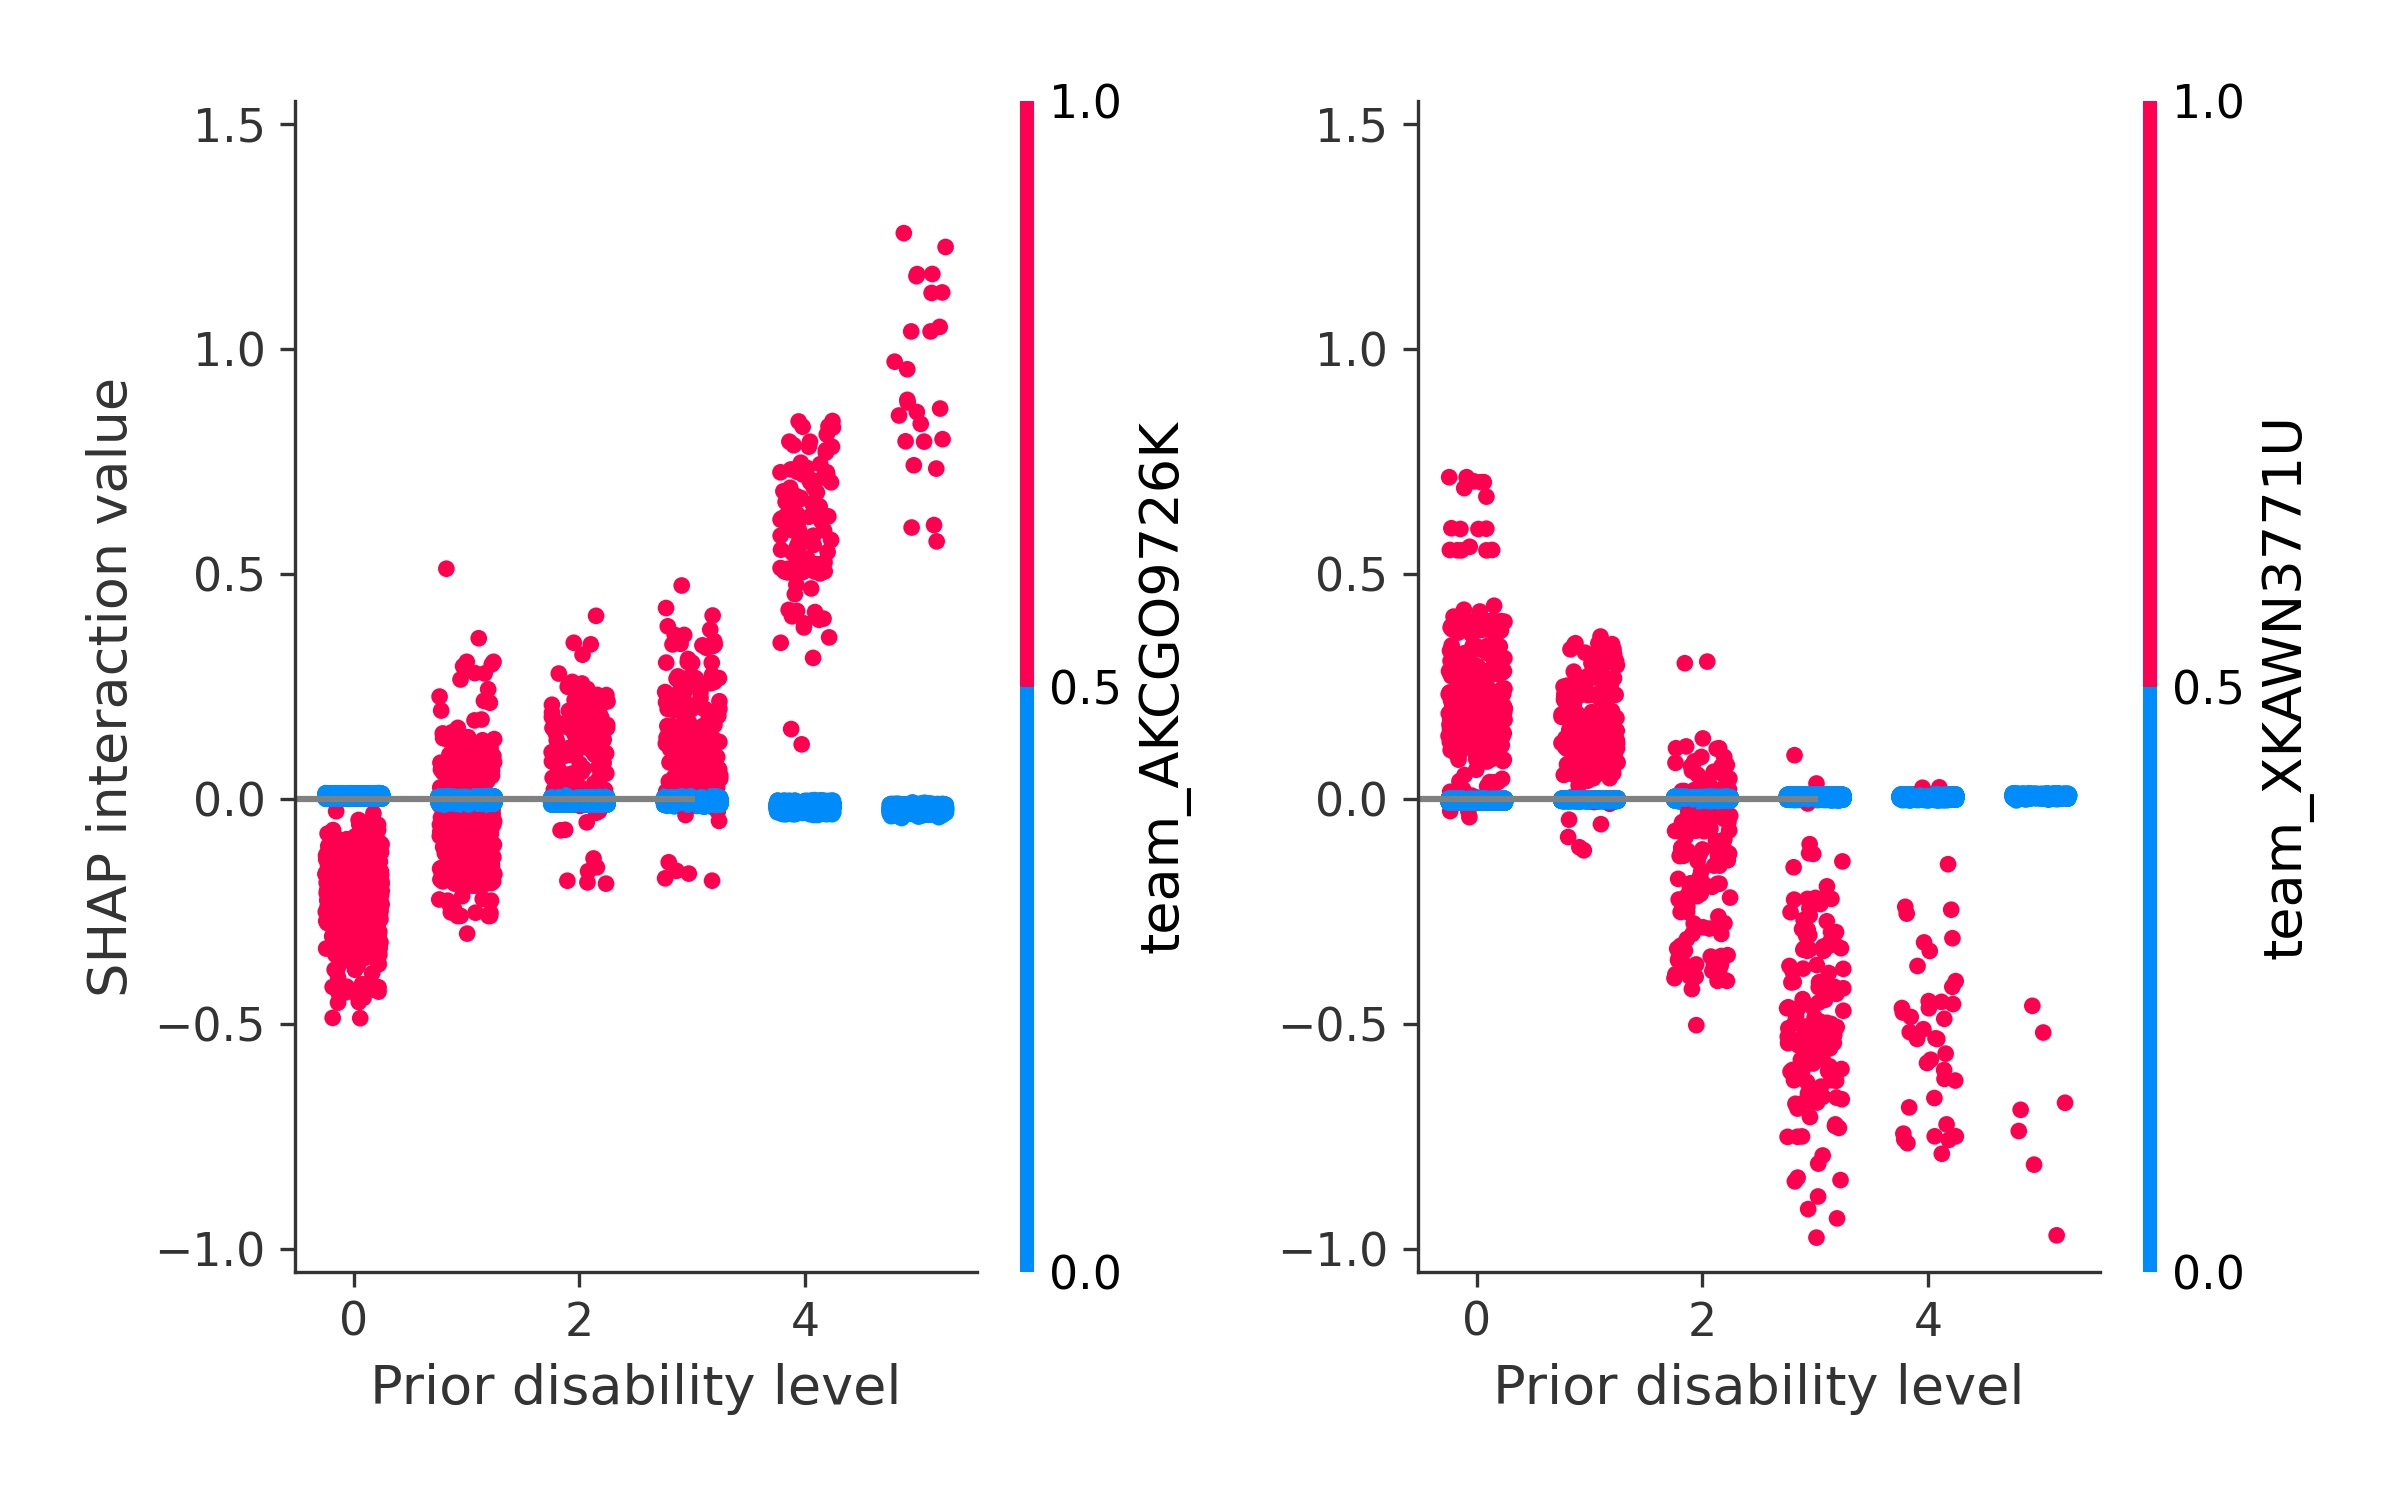
\includegraphics[width=0.75\textwidth]{./images/12ac_disability_interaction_example}
    \caption{}
    \label{fig:results_8}
    \end{figure}
    
    
    \newpage
    
    \begin{figure}[!h]
    \centering
    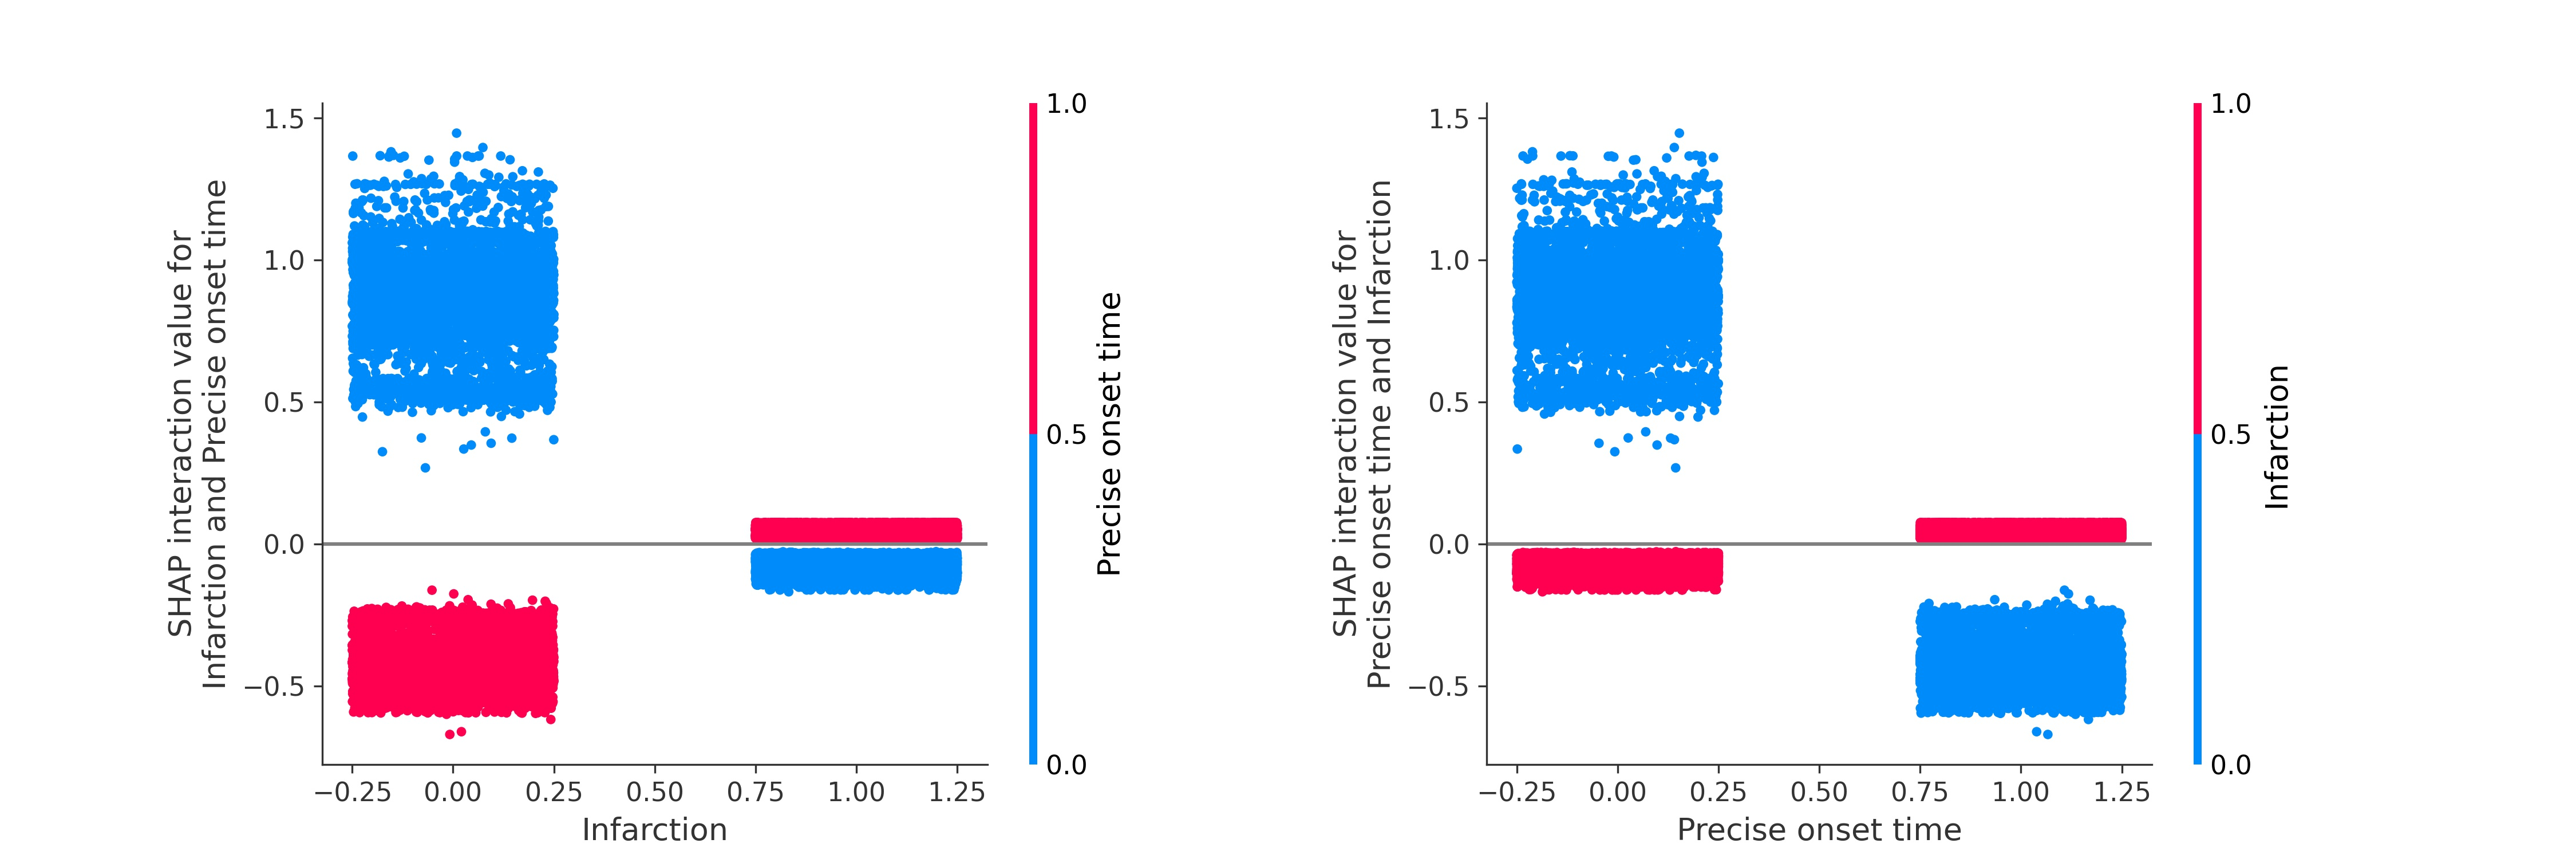
\includegraphics[width=0.75\textwidth]{./images/shap_interaction_scatter_Infarction_Precise onset time}
    \caption{}
    \label{fig:results_10}
    \end{figure}
    
\fi

